\chapter{\textit{CP} parameters measurement}
The measurement of $\it{CP}$ parameters requires the fit to the time-dependent distribution of events based on the decay time difference, flavor, and $\it{CP}$ parameters, in which $\Delta t$ is decay time difference and q is flavor of tag-side meson. $q = \pm 1$ when tag-side is $B^0$ or $\bar{B^0}$. The physical distribution of events satisfies the function in Eq(5.1), where we use the notations that is slightly different than Chapter 1. The $S_f$ and $A_f$ which stand for mixing induced and direct $\it{CP}$ violation that are noted as $\mathcal{S}$ and $\mathcal{A}$.

\begin{equation}
\mathcal{P}_{sig}(\Delta t, q ) = 
\frac{e^{-|\Delta t|/\tau_{B^0}}}{4\tau_{B^0}}
\begin{Bmatrix}
1 + q \cdot 
\begin{bmatrix}
\mathcal{S}sin(\Delta M_d \Delta t) + 
\mathcal{A}cos(\Delta M_d \Delta t)
\end{bmatrix}
\end{Bmatrix}
\end{equation}

In above function, it's parameterized by $\mathcal{S}$ and $\mathcal{A}$.
A complete model that includes the overlay of background components and outlier bands can be defined as : 

\begin{equation}
\begin{split}
\mathcal{P}(\Delta t_i,q_i,f_i^{sig},\mathcal{S},\mathcal{A})
&=(1-f_{ol})\begin{bmatrix}f_{sig}\mathcal{P}_{sig}(\Delta t_i,q_i,\mathcal{S},\mathcal{A})+(1-f_{sig}\mathcal{P}_{bkg}(\Delta t_i))
\end{bmatrix}\\
&+f_{ol}\mathcal{P}_{ol}(\Delta t_i)
\end{split}
\end{equation}

where $\mathcal{P}_{bkg}$ and $\mathcal{P}_{ol}$ are defined by: 

\begin{equation}
\mathcal{P}_{bkg} (\Delta t_i)=
f_{bkg}^{\delta}\delta(\Delta t_i-\mu_{bkg}^{\delta})+(1-f_{bkg}^{\delta})
\frac{1}{2\tau_{bkg}}e^{-|\Delta t_i-\mu_{\tau}^{bkg}|/\tau_{bkg}}
\end{equation}

\begin{equation}
\mathcal{P}_{ol} (\Delta t_i)=
G(\Delta t_i, \sigma_{ol})
\end{equation}

$\delta(\Delta t_i-\mu_{bkg}^{\delta})$ is Dirac type $\delta$ function. Eq(5.2) is using $\Delta t_i$ as i-th event's  decay time difference $\Delta t_i = \Delta z / \beta\gamma c$ in data set, where $\Delta z = z_{cp}-z_{tag}$. 

\section{Vertex Resolution Model}
\subsection{$\it{CP}$-side resolution function}
Eq(5.2) presents an ideal distribution of $\Delta t_i$ without considering the difference between measured vertex position and the physical ones. The difference can be described by introducing resolution functions. If considering resolution function, Eq(5.2) turns into: 
\begin{equation}
\begin{split}
\mathcal{P}(\Delta t_i,q_i,f_i^{sig},\mathcal{S},\mathcal{A})
&=(1-f_{ol})\text{[}f_{sig}\mathcal{P}_{sig}(\Delta t_i)\circledast R_{sig}(\Delta t_i)\\
&+(1-f_{sig})\mathcal{P}_{bkg}(\Delta t_i)\circledast R_{bkg}(\Delta t_i)
\text{]}\\
&+f_{ol}\mathcal{P}_{ol}(\Delta t_i)\circledast R_{ol}(\Delta t_i)
\end{split}
\end{equation}

$R_{sig}$ stands as resolution function for signal component, which receives smearing effect from \textit{CP} and tag side, namely $R_{cp}$ and  $R_{tag}$. The treatment of \textit{CP} side and tag side is different because of vertexing strategies. For \textit{CP} side, vertex of $B^0$ is reconstructed by fully fitting all the daughter particles. Instead, in tag side, there's no reconstruction of $B^0$ so vertex fit is performed by geometric fitting with selected charged tracks. The background events has its own resolution model which is independent from any $\it{CP}$ violation parameters. The outlier is used to compensate and smooth the long tails when $\Delta t$ becomes very large. In this analysis, we don't include the outlier to have a more realistic model under very low statistics. 


Considered only the detector effect on vertex difference along z-axis $\Delta z$. 

\begin{equation}
\Delta z 
=\Delta z^{'} + (z_{cp}^{}- z_{cp}^{'}) - (z_{tag}^{}- z_{tag}^{'}) 
\end{equation}where the primed ones stands for physical truth of position and the non-primed is measured. Footnotes are from either \textit{CP} side or tag side position. The resolution function clearly comes from $\it{CP}$ and tag-side, so for signal events, we determine the resolution models from $\it{CP}$ and tag-side separately. The resolutions on both sides also depends on the fitting method and the applied constraint, so to generalize the options used, there's no IP constraint from both side when the vertex is fitted, which avoids potential bias from  IP profile under this low statistical situation.

%\begin{equation}
%R_{sig}=R_{cp}( z_{cp}- z_{cp}^{'})\circledast
%R_{tag}( z_{tag}- z_{tag}^{'})
%\end{equation}
$\it{CP}$-side vertex is fitted with TreeFit as mentioned in the previous section where all tracks from a reconstructed event is used, thus the resolution models only depends on detectors' performance. For the $\it{CP}$-side vertex from TreeFit, the vertex resolution has relation towards the reconstruction quality, or to be more specific, the $\chi_2/N$ value, which $\chi_2$ represents the goodness of fit and N is the fitting's degree of freedom. The distribution of $\chi_2/N$ (called as reduced $\chi_2$) in selected events are shown below: 

\begin{figure}[H]
	\centering
	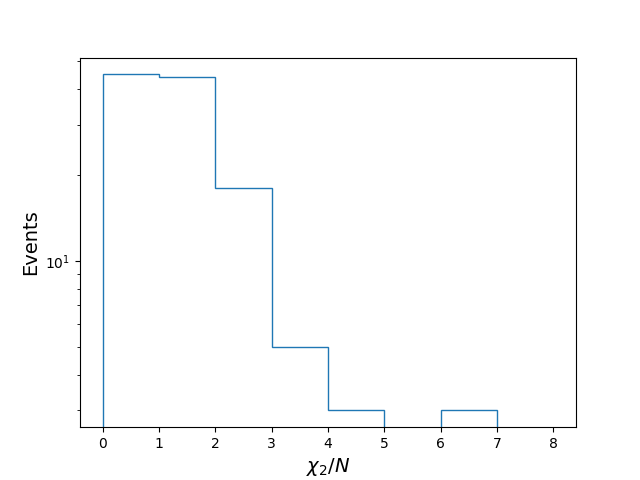
\includegraphics[height=6cm]{redChi2.png}
	\caption{$\chi_2/N$ of selected events from data.}
\end{figure}

Based on this, we model the resolution functions on $\it{CP}$-side vertexing using a double-gaussian function, whose mean is set to zero and the standard deviation is scaled by $\chi_2/N$ and the error of vertexing. 

\begin{equation}
R_{cp}(\delta z_{cp}) = (1-f_{cp}^{tail})G(0,s_{cp}^{main})+
f_{cp}^{tail}G(0,s_{cp}^{tail})
\end{equation} where: 

\begin{eqnarray}
\begin{split}
s_{cp}^{main}&=(s_0^{main} + s_1^{main}\cdot \chi^2_{cp}/NDF )\cdot \sigma_{z_{cp}}\\
s_{cp}^{tail}&=(s_0^{tail} + s_1^{tail}\cdot \chi^2_{cp}/NDF )\cdot \sigma_{z_{cp}}
\end{split}
\end{eqnarray} 
The dependence of resolution models on $\chi_2/N$ is shown as follows. Restrictively speaking, the $\it{CP}$-side resolution for $B^0 \to K_S^0  K_S^0  K_S^0$ is slight different from other channels such as $B^0\to J/\psi K_S^0$, due to the lack of the direct charged tracks from the $B^0$ vertex. The way of scaling the resolution will be further studied along with more data available. Given the current low statistics, the above model works well as an approximation. By fitting the resolution functions from signal MC on $\it{CP}$-side, we could determine the parameters in Eq(5.7), and it's listed in Table 5.1.
\begin{figure}[H]
	\begin{subfigure}{0.5\linewidth}
		\caption{$0<\chi_2/N<10$}
		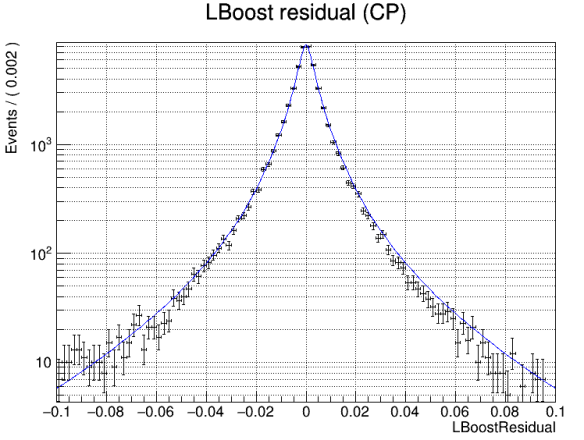
\includegraphics[height=5cm]{figures/residual0_10}
		
	\end{subfigure}
	\begin{subfigure}{0.5\linewidth}
		\caption{$0<\chi_2/N<0.4$}
		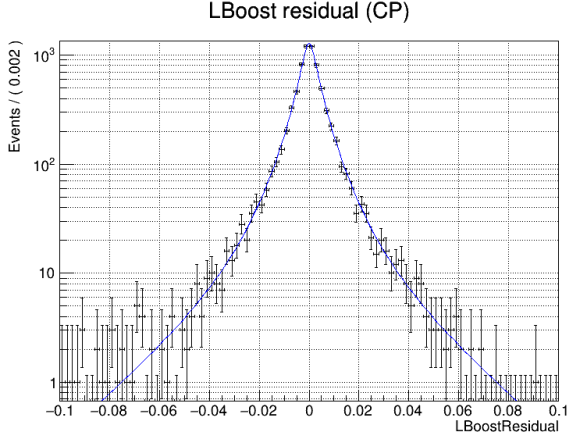
\includegraphics[height=5cm]{figures/residual0_0.4}
		%\caption{Tagging efficiency $\epsilon$ and $\mu$ in r-bins for $B^0 \to K_S^0  K_S^0  K_S^0$.}
	\end{subfigure}
	
	
	\begin{subfigure}{0.5\linewidth}
		\caption{$0.4<\chi_2/N<0.8$}
		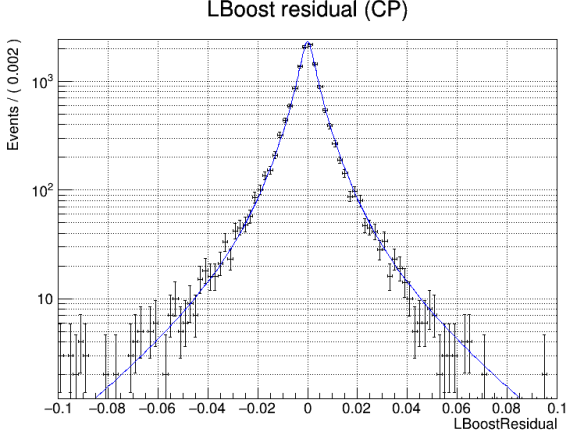
\includegraphics[height=5cm]{figures/residual0.4_0.8}
		%\caption{Tagging efficiency $\epsilon$ and $\mu$ in r-bins for $B^0 \to K_S^0  K_S^0  K_S^0$.}
	\end{subfigure}
	\begin{subfigure}{0.5\linewidth}
		\caption{$0.8<\chi_2/N<1.2$}
		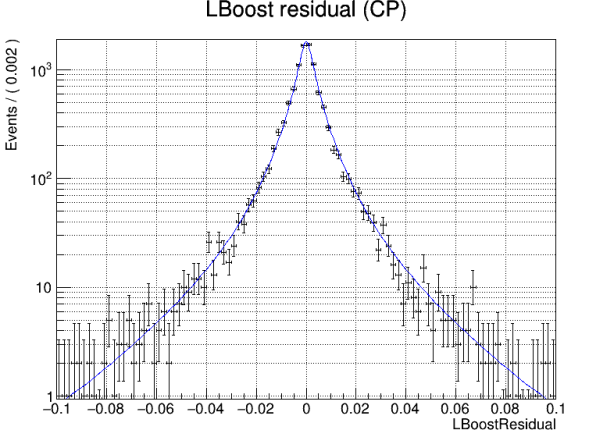
\includegraphics[height=5cm]{figures/residual0.8_1.2}
		%\caption{Tagging efficiency $\epsilon$ and $\mu$ in r-bins for $B^0 \to K_S^0  K_S^0  K_S^0$.}
	\end{subfigure}
	
	\begin{subfigure}{0.5\linewidth}
		\caption{$1.2<\chi_2/N<1.6$}
		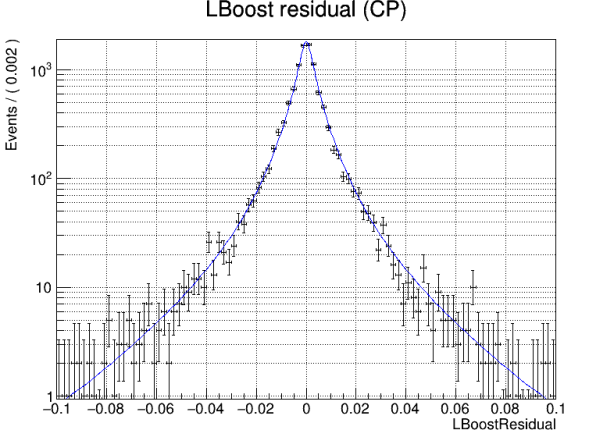
\includegraphics[height=5cm]{figures/residual1.2_1.6}
		%\caption{Tagging efficiency $\epsilon$ and $\mu$ in r-bins for $B^0 \to K_S^0  K_S^0  K_S^0$.}
	\end{subfigure}
	\begin{subfigure}{0.5\linewidth}
		\caption{$1.6<\chi_2/N<10$}
		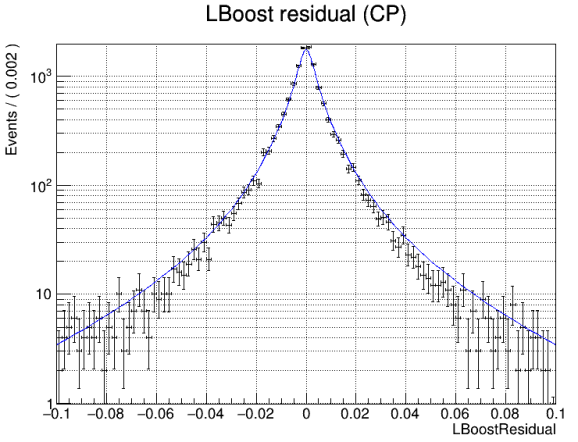
\includegraphics[height=5cm]{figures/residual1.6_10}
		%\caption{Tagging efficiency $\epsilon$ and $\mu$ in r-bins for $B^0 \to K_S^0  K_S^0  K_S^0$.}
	\end{subfigure}
	\caption{Resolution functions on $\it{CP}$-side, which shows dependence on the $\chi_2/N$}
\end{figure}

\begin{table}[H]
	\begin{minipage}[b]{1.0\linewidth}
		\centering
		\caption{Parameters in $R_{cp}$.}
		\begin{tabular}{|c|c|}
			\hline
			$f_{cp}^{tail}$ & $0.07424 \pm 0.0008$\\
			$s_0^{main}$&  $0.9151 \pm 0.0077$ \\
			$s_1^{main}$ & $0.2142\pm 0.0064$\\
			$s_0^{tail}$ &  $2.0477\pm 0.0779$\\
			$s_1^{tail}$  & $1.3470\pm 0.0720$ \\
			\hline
		\end{tabular}
	\end{minipage}
\end{table}

\subsection{Tag-side resolution function}

For the tag-side, the vertexing is done by using KFit and No IP constraint. Since we don't reconstruct certain decay channel like $\it{CP}$-side, there's no guarantee that tracks used by KFit are all from the primary vertex. This leads to the resolution degradation on tag side vertexing called $R_{np}$. To the contrary, if all tracks that are used for tag vertexing are from primary vertex, then resolution will only be affected by the detector, and this is called $R_{det}$, similarly to $R_{cp}$. The model is demonstrated as below:
\begin{equation}
\begin{split}
z_{tag} - z_{tag}^{'} =& z_{tag}^{'} + \delta z_{tag}^{det} + \delta z_{tag}^{np} - z_{tag}^{'}\\
=&\delta z_{tag}^{det} + \delta z_{tag}^{np}
\end{split}
\end{equation}
\begin{equation}
R_{tag}( z_{tag}- z_{tag}^{'}) = R_{det}^{tag}(\delta z_{tag}^{det}) \circledast
R_{np}^{tag}( \delta z_{tag}^{np})
\end{equation}

\begin{equation}
R_{det}^{tag}(\delta z_{tag}^{det}) = (1-f_{tag}^{tail})G(0,s_{tag}^{main}\cdot\sigma_{z_{tag}})+
f_{tag}^{tail}G(0,s_{tag}^{tail}\cdot\sigma_{z_{tag}})
\end{equation} where main and tail parts share same main value at zero, but deviation is defined by using uncertainties in each event $\chi^2_{tag}/N$: 

\begin{equation}
s_{tag}^{main/tail} = s_0^{main/tail} + s_1^{main/tail}\cdot\chi^2_{tag}/NDF
\end{equation} where $\chi^2_{tag}/N$ is returned by tag side vertexing tool on event-by-event basis.
Technically $R^{tag}_{det}$ can be fitted with MC of which tag side tracks are all from primary vertex. Then after fixing the fitted parameters of $R^{tag}_{det}$ , $R^{tag}$ will only be dependent on $R^{tag}_{np}$. 

As for the fit of $R_{np}$, similar event-by-event fit is also implemented. The fit model of $R_{np}$ is inherited Belle experience. It consists of three functions, including one Dirac type $\delta$ function and two single side exponential. 

\begin{equation}
R_{tag}^{np}(\delta z_{tag}^{np})=f_{\delta}\delta(\delta z_{tag}^{np}) + 
(1-f_{\delta})[f_p E_p(\delta z_{tag}^{np},\tau_p\cdot \sigma_{z_{tag}}) +
(1-f_p)E_n(\delta z_{tag}^{np},\tau_n\cdot \sigma_{z_{tag}}) ]
\end{equation} where $E_p(x,\tau_p)=(1/\tau_p)exp(-x/\tau_p) $ when $x > 0$ and $E_n(x,\tau_n)=(1/\tau_n)exp(x/\tau_n) $ when $x < 0$.

Also, since tag-side has no dependence of how $\it{CP}$-side decays, its resolution is almost mode-independent. We use the parameters that is obtained by fitting to the control sample data. The details about control sample study are here\cite{jpsiks_ichep}. The fit results for tag-side resolution is shown in Fig 5-3 and 5-4 and Table 5.3 and Table 5.4.

\begin{table}[H]
	\begin{minipage}[b]{1.0\linewidth}
		\centering
		\caption{Parameters in $R_{cp}$.}
		\begin{tabular}{|c|c|}
			\hline
			$f_{cp}^{tail}$ & $0.07424 \pm 0.0008$\\
			$s_0^{main}$&  $0.9151 \pm 0.0077$ \\
			$s_1^{main}$ & $0.2142\pm 0.0064$\\
			$s_0^{tail}$ &  $2.0477\pm 0.0779$\\
			$s_1^{tail}$  & $1.3470\pm 0.0720$ \\
			\hline
		\end{tabular}
	\end{minipage}
\end{table}

\begin{figure}[H]
	\begin{minipage}[b]{0.5\linewidth}
		\centering
		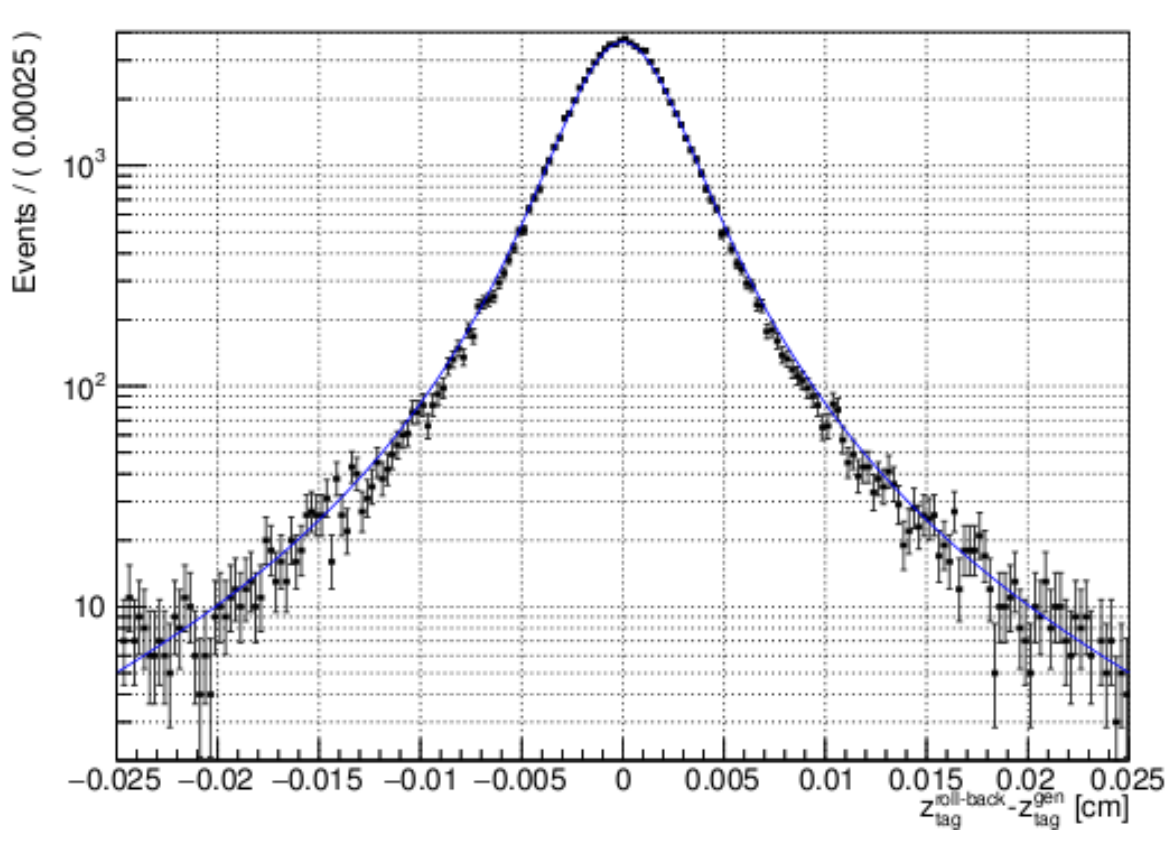
\includegraphics[height=5cm]{figures/Rdet}
		\caption{$R_{det}^{tag} $ fit}
	\end{minipage}
	\begin{minipage}[b]{0.5\linewidth}
		\centering
		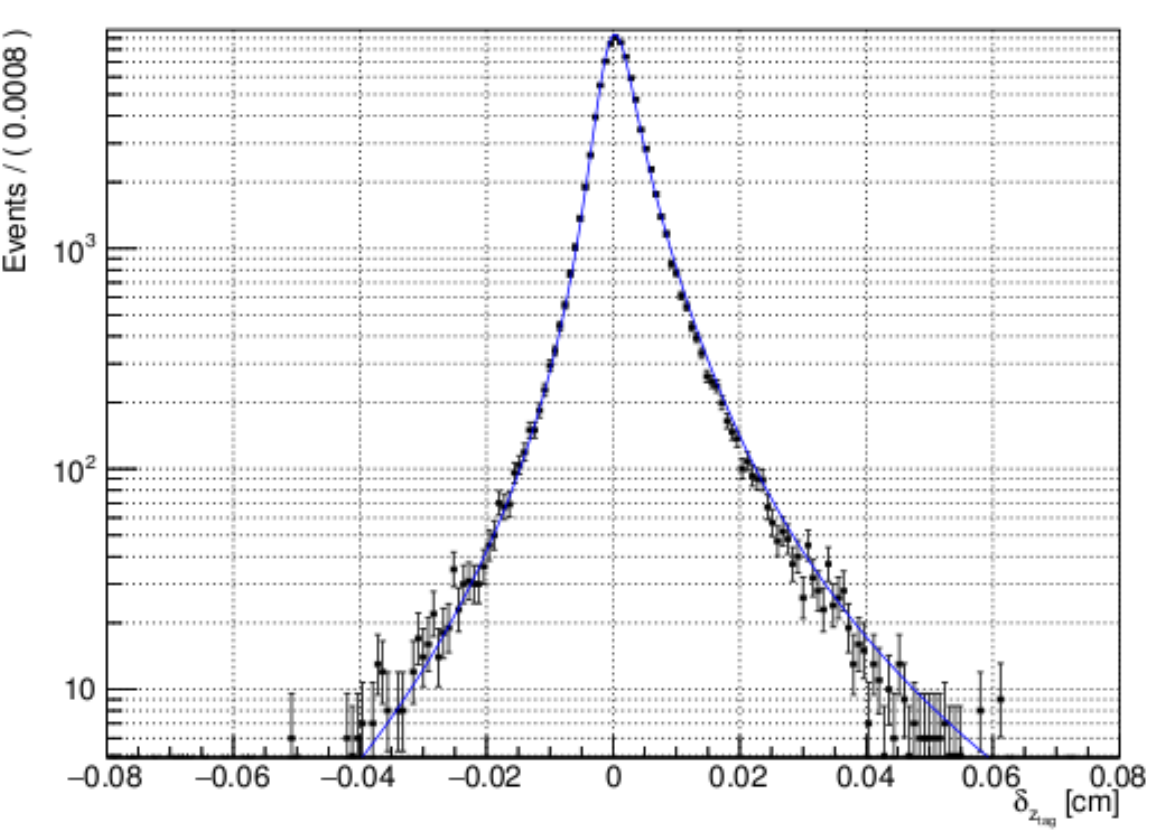
\includegraphics[height=5cm]{figures/Rnp}
		\caption{$R_{np}^{tag}$ fit}
	\end{minipage}
\end{figure}
\begin{table}[H]
	\begin{minipage}[b]{0.5\linewidth}
		\centering
		\caption{Parameters in $R^{tag}_{det}$}
		\begin{tabular}{|c|c|}
			\hline
			$f_{tag}^{tail}$ & $0.0523 \pm 0.0025$\\
			$s_0^{main}$&  $1.1446 \pm 0.0061$ \\
			$s_1^{main}$ & $0.0443\pm 0.0022$\\
			$s_0^{tail}$ &  $3.4480\pm 0.0897$\\
			$s_1^{tail}$  & $0.2666\pm0.0276$ \\
			\hline
		\end{tabular}
	\end{minipage}
	\begin{minipage}[b]{0.5\linewidth}
		\centering
		\caption{Parameters in $R^{tag}_{np}$}
		\begin{tabular}{|c|c|}
			\hline
			$f_{\delta}$ & $0.6256\pm 0.0049$\\
			$f_p$ &  $0.8316 \pm 0.0051$ \\
			$\tau_n$ & $2.9141\pm 0.0758$\\
			$\tau_p$ &  $2.4846\pm 0.0269$\\
			\hline
		\end{tabular}
	\end{minipage}
\end{table}


 Last but not least, the boost direction of each event is not constant event-by-event, so the z-axis position of vertex may not be optimized by calculating  $\Delta t_i = \Delta z / \beta\gamma c$. This effect can be reduced by replacing z position with the relative distance along the boosting direction, or introducing another resolution function called $R_k$. In the current modeling of Belle II tag side resolution, distance along the boost direction is available so $R_k$ is not yet implemented. So we use the $\Delta Z$ projection on the boosted direction of each event to account for this effect when we define the parameters of resolution and also for the final fit to Eq(5.5).



\subsection{Background events distribution}
Instead, $R_{bkg}$ is in a simpler shape and it's uncorrelated to vertexing method approximately. Because the source of background mainly comes from continuum events passing the selection, it's reasonable to model its resolution by Gaussian-like function. We define a double-Gaussian with its standard deviation scaled by the measured uncertainties from both sides as Eq(5.14) shows. 

\begin{equation}
R_{bkg} = (1-f^{bkg}_{tail})G(\Delta t_i, \sigma^{bkg}_{main}\sqrt{\sigma^2_{cp}+\sigma^2_{tag}})
+ f^{bkg}_{tail}G(\Delta t_i, \sigma^{bkg}_{tail}\sqrt{\sigma^2_{cp}+\sigma^2_{tag}})
\end{equation} It convolution integrals with $\mathcal{P}_{bkg}$:

\begin{equation}
\mathcal{P}_{bkg}=f_{\delta}^{bkg}\delta(\Delta t - \mu^{bkg}_{\delta})+
(1-f_{\delta}^{bkg})\frac{1}{2\tau_{bkg}}e^{-|\Delta t - \mu^{bkg}_{\tau}|/\tau_{bkg}}
\end{equation}
With this definition, one can make background component $\mathcal{P}_{bkg}\circledast R_{bkg}$ and fit to side-band data to obtained the parameters. There are total seven parameters in float to determine which are listed down below with primary fit results on sideband data, which according to the previous section, is totally 60 events in $M_{bc} <5.26$ GeV.

\begin{figure}[H]
	%	\begin{minipage}[b]{0.5\linewidth}
	%		\centering
	%		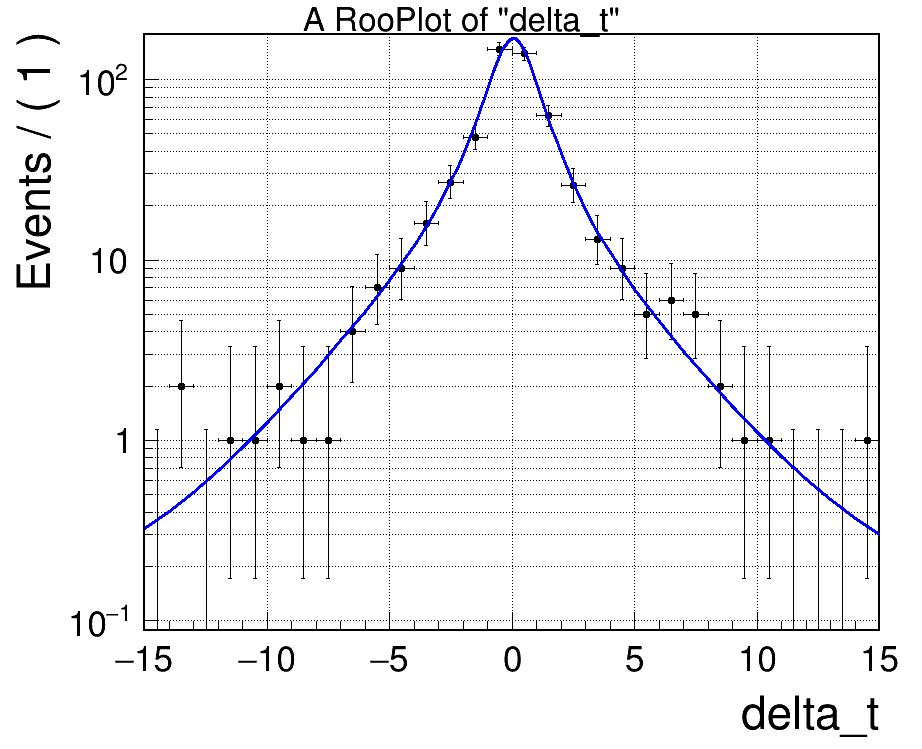
\includegraphics[height=5cm]{figures/bkg-cpfit-gen-mbc526}
	%		\caption{Background fit on generic sideband}
	%	\end{minipage}
	%	\begin{minipage}[b]{0.5\linewidth}
	\centering
	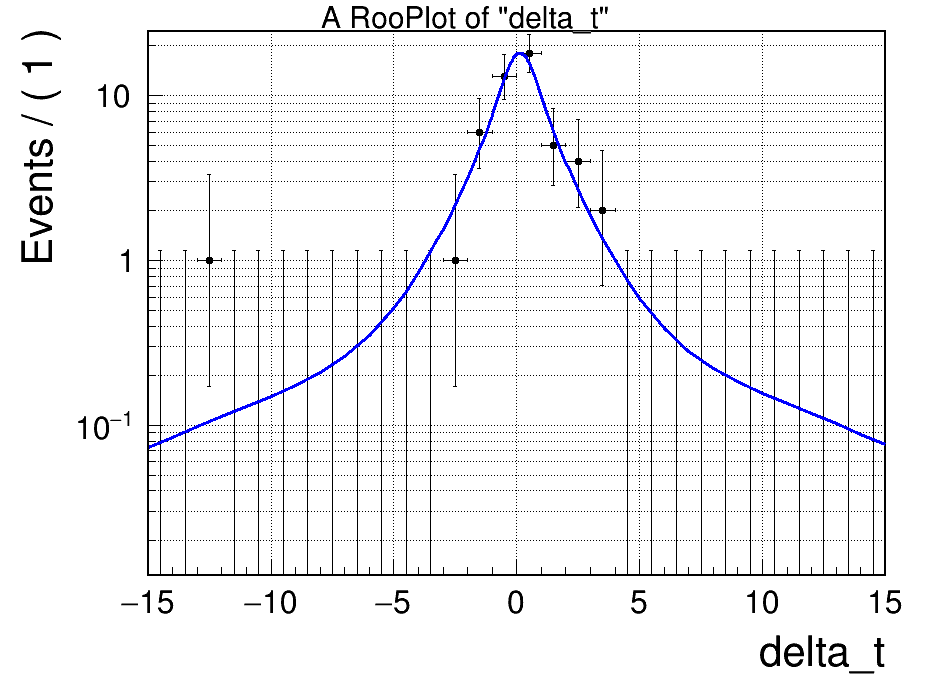
\includegraphics[height=5cm]{figures/bkg-cpfit-data-mbc526}
	\caption{Background fit on data sideband with $M_{bc} < 5.26 GeV$}
	%	\end{minipage}
\end{figure}
\begin{table}[H]
	\centering
	\begin{tabular}{|c|c|}
		\hline
		$\mu^{bkg}_{\delta}$ & $0.1310 \pm 0.1902$\\
		$\mu^{bkg}_{l}$&  $0.1638 \pm 0.5030$ \\
		$\tau_{bkg}$ & $1.0541\pm 0.4370$\\
		$f_{\delta}^{bkg}$ &  $0.5861\pm 0.2570$\\
		$f^{bkg}_{tail}$  & $0.0417\pm 0.0408$ \\
		$\sigma^{bkg}_{main}$ & $1.4348\pm 0.3940$\\
		$\sigma^{bkg}_{tail}$ & $28.0930 \pm 8.8221$\\
		\hline
	\end{tabular}
	\caption{Parameters in Background $\Delta t$ distribution. }
\end{table}


\section{Flavor Tagging}
 In order to determine the flavor of tag side $B^0$, flavor tagging algorithm is being developed. The tagger uses information from $\mu^{\pm}$, $\pi^{\pm}$,$K^{\pm}$ and $\Lambda^{}$ and categorized them into 13 different types as illustrated below. 

\begin{figure}[H]
\centering
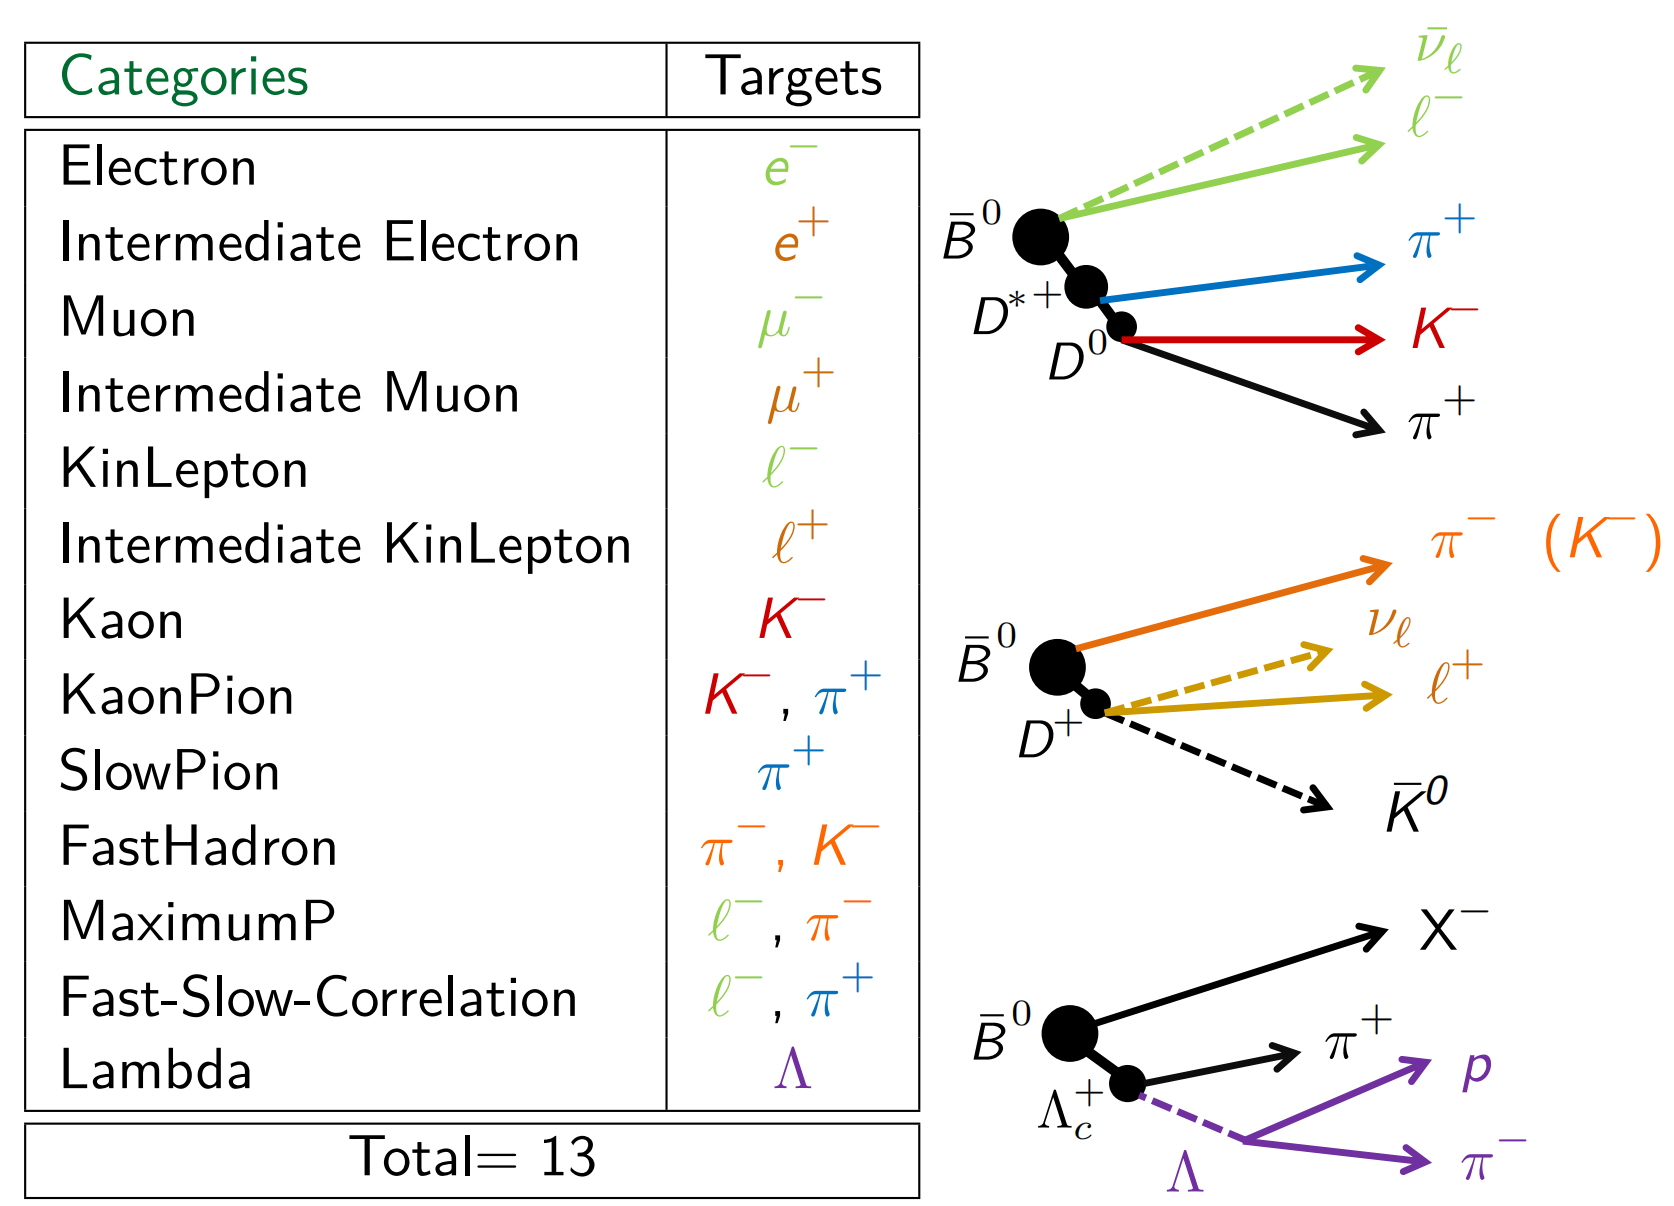
\includegraphics[width=0.7\linewidth]{tagger}
\caption{Particles and their categories used in flavor tagging algorithm.}
\end{figure}
 
 
For each particle that has been used from above categories, PID and kinematics (such as $p_t$,$cos\theta$,$d_0$,etc) information are extracted and feed to the combiner as training variables, to form a output corresponding each category. Then for all outputs from these categories, a total classifier is trained to present the likelihood of flavor $q$. This algorithm is called category-based algorithm which is used in our analysis. Similar tagger based on deep neural-network algorithm is also available but will not be further discussed here. After the reconstruction on the \textit{CP} side is done, ROE objects that contains the tracks from tag side is formed, and tracks that will be used to fill the above particle lists are selected. Just like $K_S^0$ finder and continuum suppression, we choose FastBDT as classifier back-end algorithm. Targeted variable is $q$ of tag side in MC truth. The ROE selection is affected by the cleanness of \textit{CP} reconstruction, but flavor tagging should be almost mode-independent. To minimize impact of the reconstruction performance, MC sample of $B^0 \to \nu \nu$ is used for training the tagger where \textit{CP} side is completely invisible. Then the trained classifier can be applied to signal sample.

 The statistical uncertainty of $\mathcal{S}$ now receives contribution from $\epsilon$ and $w$: $\delta(\mathcal{S}) \propto \frac{1}{\epsilon (1-2w)N_{rec}}$, which make it crucial to correctly measure tagging efficiency and wrong tag fraction. $w$ can be estimate using MC sample which the bias on individual events could propagate to the fit of $\mathcal{S}$. By measuring $w$ from flavor specific decay using real data, bias from MC can be avoid. The validation of flavor tagger using flavor specific control sample is summarized here: \cite{flavortagger}. For flavor specific decay, the Eq(5.17) and Eq(5.18) could be used to fit the wrong tagging fraction and efficiency.
 
 \begin{equation}
 \mathcal{P}_{SF/OF}^{obs}(\Delta t, q_{cp},q_{tag}, \epsilon, w) = 
 \frac{e^{-|\Delta t|/\tau_{B^0}}}{4\tau_{B^0}}
 \epsilon
 \begin{bmatrix}
 1 + q_{cp}\cdot q_{tag}(1-2w)\cdot 
 cos(\Delta M_d \Delta t)
 \end{bmatrix}
 \end{equation} so wrong tag fraction can be measured by: 
 
 \begin{equation}
 \frac{\mathcal{P}_{OF}^{obs}-\mathcal{P}_{SF}^{obs}}{\mathcal{P}_{OF}^{obs}+\mathcal{P}_{SF}^{obs}}=(1-2w)cos(\Delta M_d \Delta t)
 \end{equation}
 
  If $w$ is extracted from MC, which is what we implemented in this analysis, bias could be reduced by using binned values of tagger output. To be more specific, saying the output of tagging classifier is $\alpha$ in range $[0,1]$, wrong tag probability of being $q= +1$ is defined as $ \beta = 1-\alpha$, and flavor tagger will eventually gives tagged flavor as $ \mathcal{F}= 1-2\beta = 2\alpha -1$. It's obvious that $\mathcal{F} < 0$ means the tagged flavor is $q=-1$ instead of $+1$. The distribution of $\mathcal{F}$ is shown in Fig 5-7 (up) from signal MC. The average efficiency of among all tag-able event is measured to be $99.92 \pm 0.01 \%$, and effective efficiency (percentage of correctly tagged events) is $31.31 \pm 0.52\%$ for $B^0$ and $31.13 \pm 0.51\%$ for $\overline{B^0}$. No clear bias on effective tagging efficiency is found considering the MC fraction of $B^0$ and $\overline{B^0}$ are $50.11\%$ and $48.89\%$ respectively.
 
 \begin{figure}[htpb]
 	\centering
 	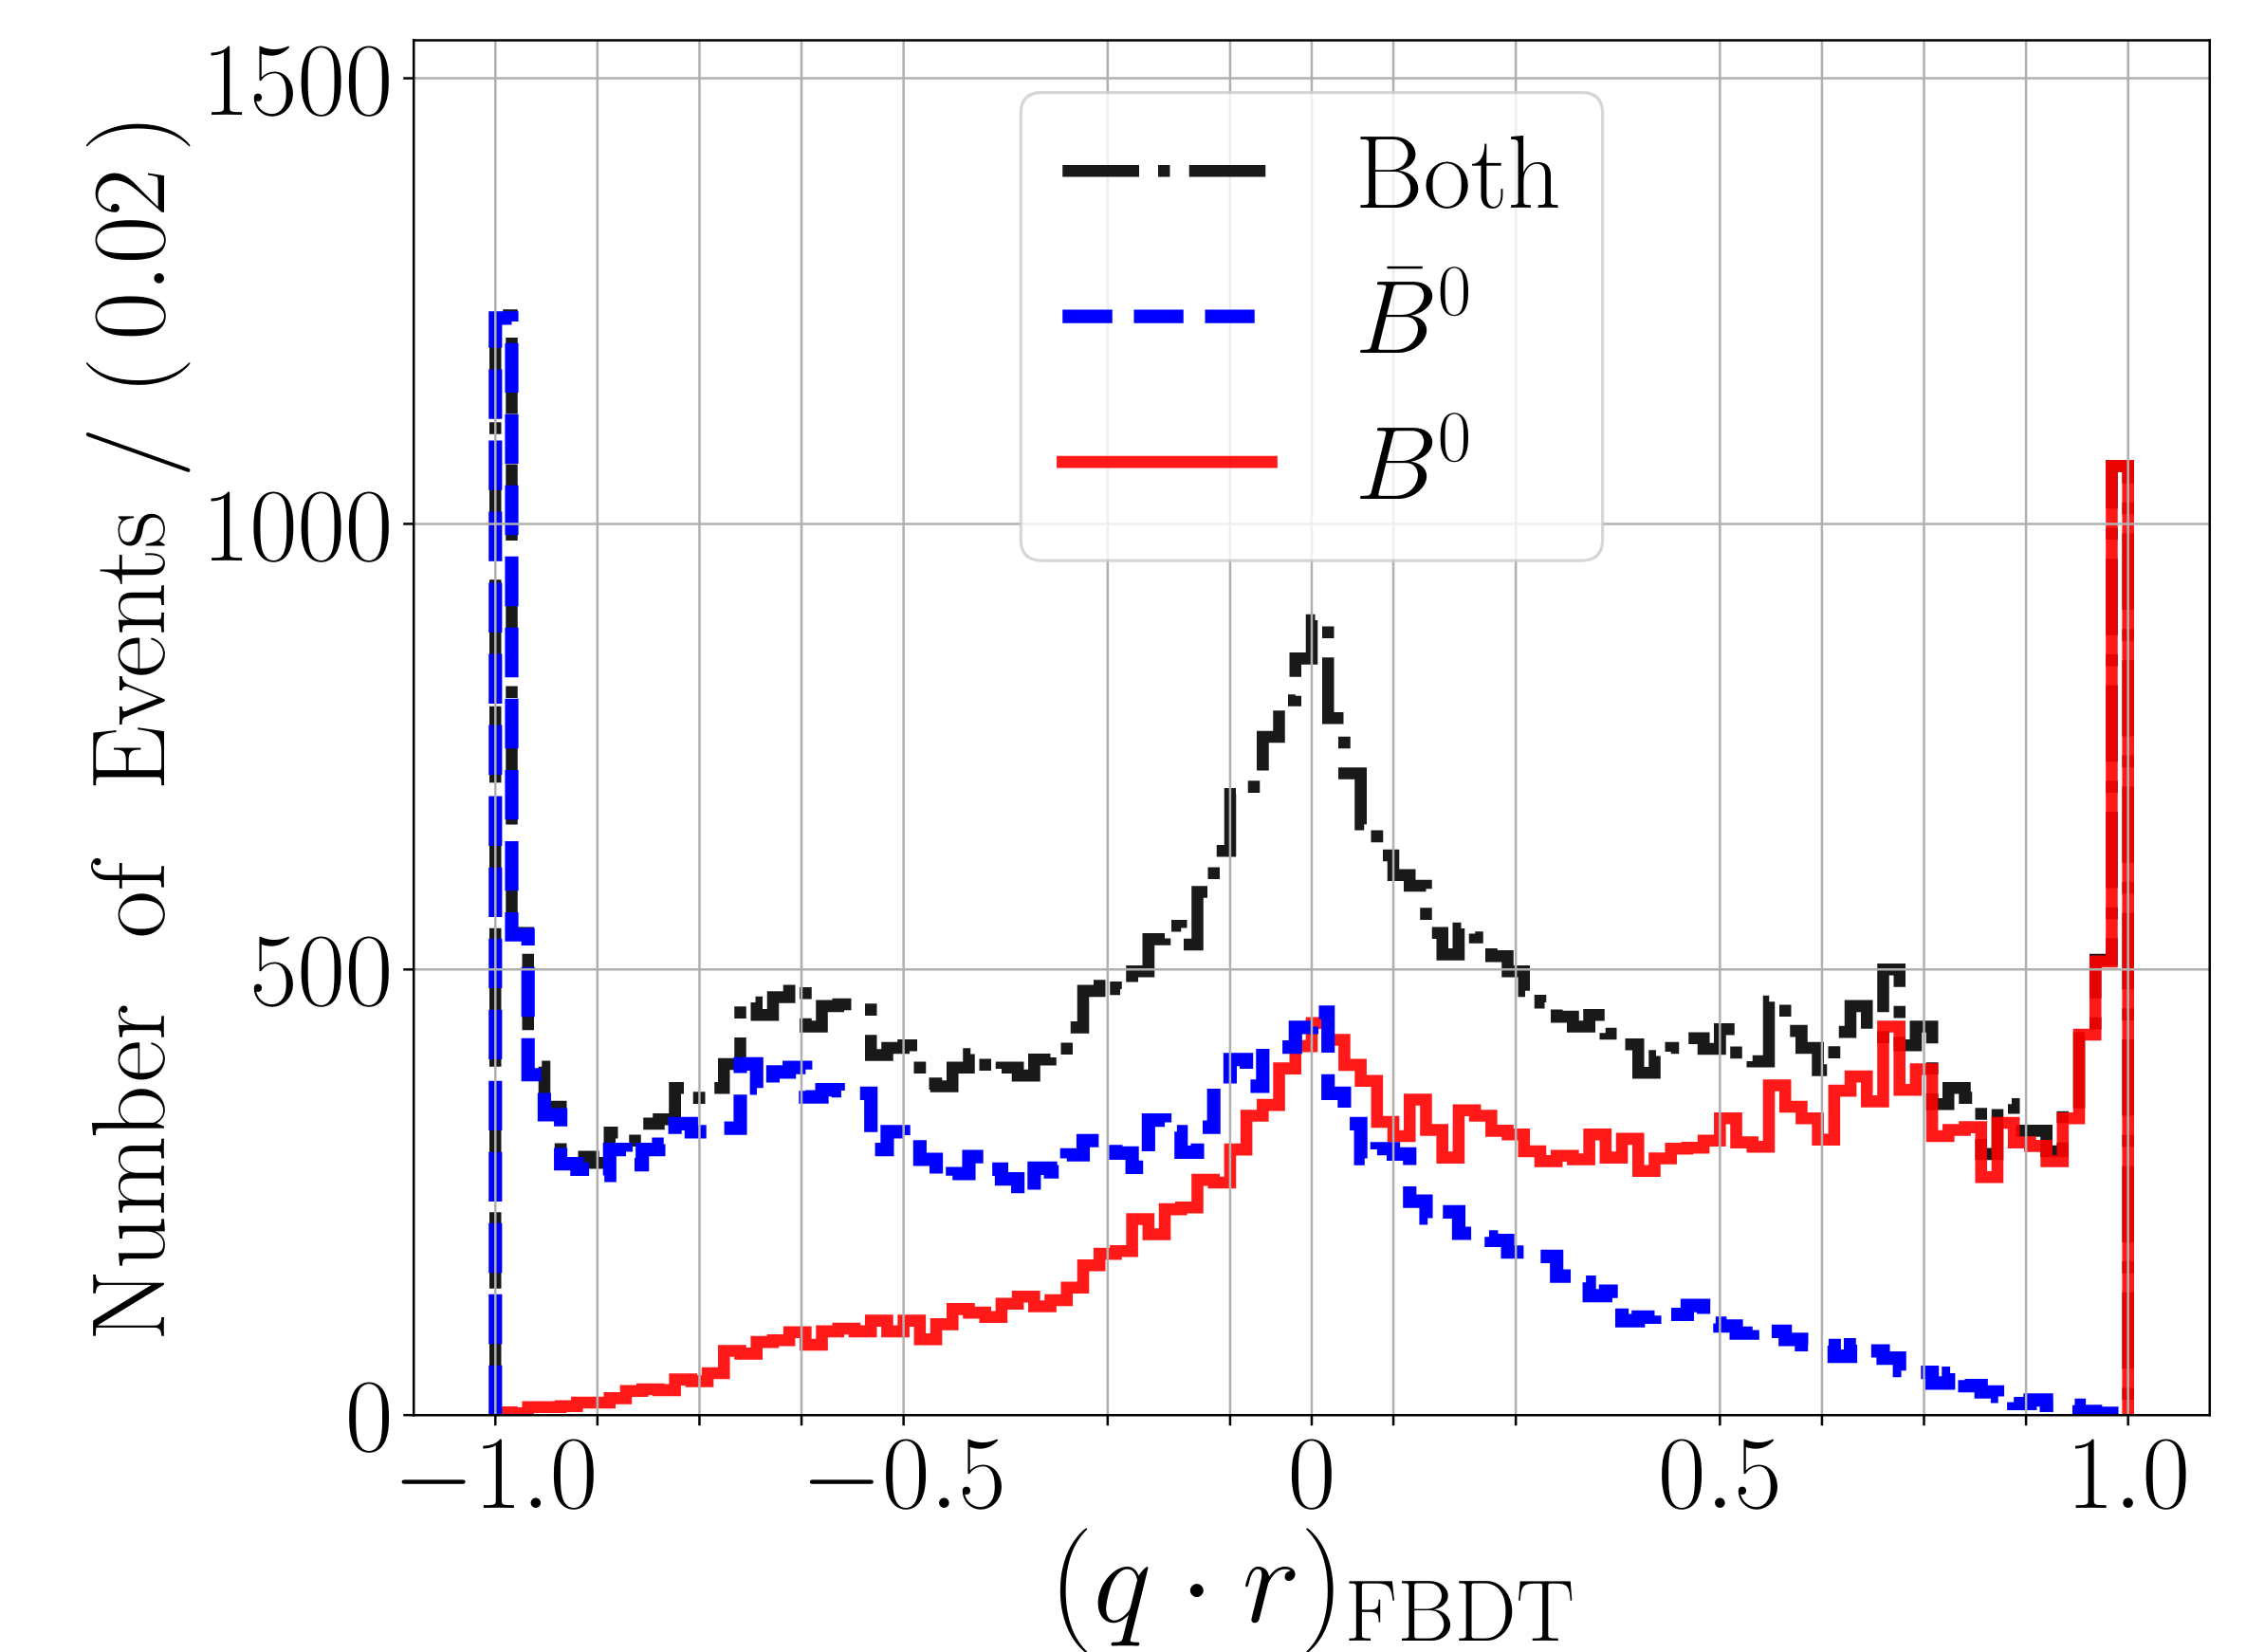
\includegraphics[width=0.7\linewidth]{figures/qr}
 	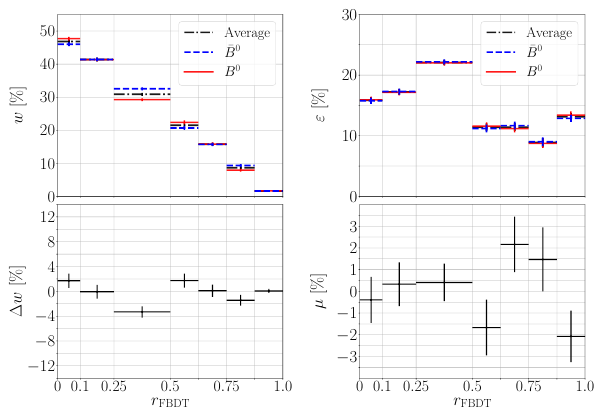
\includegraphics[height=9cm]{flavor_values}
 	\caption{Top:the distribution of flavor tagger output $\mathcal{F}=(q\cdot r)_{FBDT}$ for both tag side of $B^0$ and $\overline{B^0}$. Bottom: flavor tagging efficiency, wrong tagging fraction, tagging difference in regard to rbin.}
 	\label{fig:qr}
 \end{figure}
 
 
 The r-bins are intervals that splits the absolute value of $\mathcal{F}$, namely $r_{FBDT}=|\mathcal{F}|$, where the true flavor $q$ is irrelevant to r-bins. Belle experience on defining the r-bins is inherited where bins are set as $[0,0.1,0.25,0.5,0.625,0.75,0.875,1]$.For all MC events that have been successful tagged, they are projected into histogram of $|\mathcal{F}|$, $w$ can be calculated in each bin in the way  dividing the number of events that its $\mathcal{F}$ is opposite to its MC flavor to all the events in the same bin. The binned tagging efficiency is calculated through dividing the number of successfully tagged events by all events in the same bin. 
 
 Besides, $w$ can be different between $B^0$ and $\overline{B^0}$. Considering 
 $w = (w_{B^0}+w_{\overline{B^0}})/2$ and $\Delta w = w_{B^0}-w_{\overline{B^0}} $, so for each event of flavor $q$, it may from a correct or incorrect tagged event when we look at the distribution of Eq(5.1). 
 
 From Eq(5.1), it's obvious that the distribution of $\Delta t$ is independent from the flavor $q$, while this is not true considering the limit power of flavor tagging as we discussed. Only certain fraction of events can be flavor tagged and also only part of events are correctly tagged. Considering the effect from flavor tagging, the observed distribution of $\Delta t$ is turning into:
 
 \begin{equation}
 \mathcal{P}_{sig}^{obs}(\Delta t, q, \epsilon, w) = 
 \frac{e^{-|\Delta t|/\tau_{B^0}}}{4\tau_{B^0}}
 \epsilon
 \begin{Bmatrix}
 1 - q\cdot \Delta w+ q(1-2w)\cdot 
 \begin{bmatrix}
 \mathcal{S}sin(\Delta M_d \Delta t) + 
 \mathcal{A}cos(\Delta M_d \Delta t)
 \end{bmatrix}
 \end{Bmatrix}
 \end{equation} 
 compared to the original, the fluctuation is reduced by factor $r\equiv |1-2w|$, called as dilution factor. 
 
 As for efficiency $\epsilon$, the difference $\mu = \epsilon_{B^0}-\epsilon_{\overline{B^0}} $ is about 1\% to 2\% in each bin, thus treated as zero. The average $r$ is also calculated in r-bins. Fig 5-7 (down) shows the flavor tagging results on $w$,$\Delta w$, $\epsilon$ and $\mu$ in each of the r-bin. 
 




\section{$\it{CP}$ Fitter}

The parameters that are needed for \textit{CP} fit is basically all studied and obtainable for extracting $\mathcal{S}$ and $\mathcal{A}$ from Eq(5.2) with using observed $\Delta t$ distribution. The fit is taking the $\Delta t$, signal fraction $f_{sig}$, the flavor charge q as observables, and in the meantime the vertexing error and $\chi_2/N$ are used as event-by-event conditional variables. RooFit is configured based on this setup and unbinned maximum likelihood fit is used as the fitting strategy.
To actually perform the fit, the computation work load is an important factor to consider when the event number goes high in future.
Especially, the multiple convolution integrals of resolution model and probability density functions are a set of computing intensive works. Belle legacy fitter utilize a highly customized library called ``Tatami" to perform the convolution integrals. For Belle II, a new $\it{CP}$ fitter is developed based on Python (version 3.7) and RooFit, which is naturally easy to use and maintain with BASF2 due to BASF2's analysis controls are mostly done by Python. The code management shows a modern, good consistency and readability, which will be aimed for providing a universal fitting tool to TDCPV analysis in Belle II. The fitter requires a configuration files which contains all the observables and parameters definition including their range, value, floating state. Data that is fed to the fitter will be converted into the RooDataSet object associated with each variables from configuration file. The models of fit such as each resolution functions, signal and background P.D.F is formed with the data set in the same workspace. The convolution of each components are handled by a customized shared object written in C++ from ``SignalPdf.cxx". Combined these tools, the unbinned maximum likelihood fit is performed that can either be used to determine  $\mathcal{S}$ and $\mathcal{A}$ or other parameters when they are floating. The result of the fit then restore as ROOT files as well as corresponding plots.

\begin{figure}[H]
	\centering
	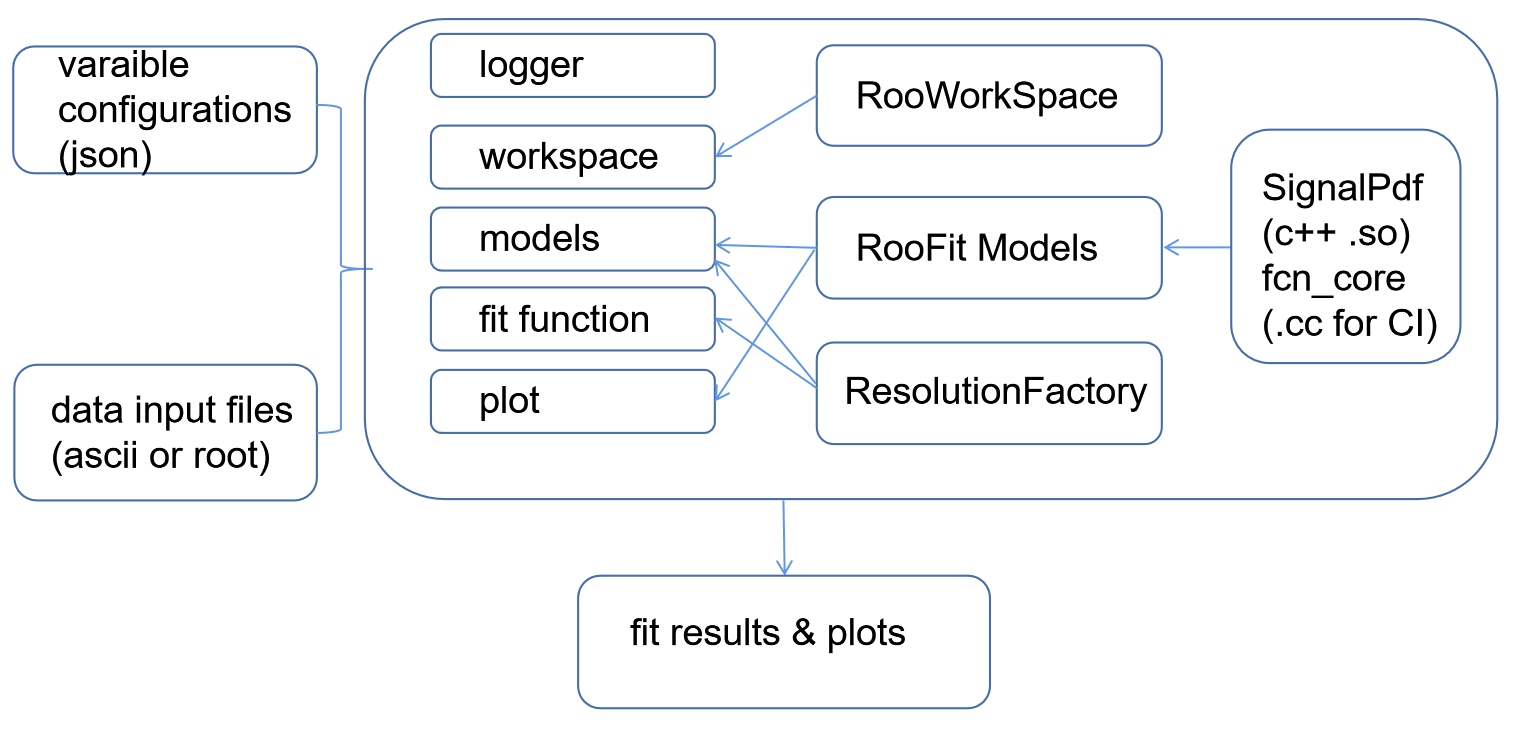
\includegraphics[height=6cm]{cpfitter-pict}
	\caption{The structure of $\it{CP}$ fitter for Belle II. Users provide configuration file containing the definitions of all parameters and observables in the $\it{CP}$ fit. Data input files are used to create dataset for fitting. External library called ``SignalPdf.cxx" are generated in runtime to calculate the integral of resolutions and physics distribution event by event, which the fit is performed by maximizing the ``fcn\_core" function, presenting the likelihood of the dataset to the fit model. }
\end{figure}



\section{Blind Fit}
As a required procedure to make sure the $\it{CP}$ parameters are measured without bias due to the preconceived results, a blind analysis procedure is conducted before the fit is actually performed using the experimental data. The blind fit procedure includes the $\it{CP}$ fit on signal MC and generic MC, with different number of events used. To check the reliablity of fit result from $\it{CP}$ fitter, a linearity test and toy MC study is also performed. 

\subsection{$\it{CP}$ fit on MC samples}
Using $\it{CP}$ fitter, we perform the $\it{CP}$ fit on events in signal MC and generic MC.
The signal and generic MC are generated with phase-space model which contains zero $\it{CP}$ violation ($\mathcal{S}=\mathcal{A}=0$) in $B^0 \to K_S^0  K_S^0  K_S^0$ channel. 
The event with following cuts are selected for $\it{CP}$ fit. 
\begin{itemize}
	\item $-70 < \Delta t < 70$ ps
	\item $0 < (\chi_2/N)_{cp} < 8 $
	\item $0 < (\chi_2/N)_{tag} < 50 $
	\item error on tag-side vertex $< 0.1 $ cm
	\item $5.27 < M_{bc} < 5.29$ GeV and $|\Delta E| < 0.1$ GeV
\end{itemize}

We have 10000 (8873 passing selection) events from signal sample and 415 (373 passing selection) events from 1ab$^{-1}$ generic sample to fit $\it{CP}$ parameters. To mimic the events number expected in data sample, we randomly take 30 events from generic sample and perform the fit as well. The fit results are shown in Fig 5-9 to Fig 5-11. 
\begin{figure}[H]
	\begin{minipage}{0.5\linewidth}
		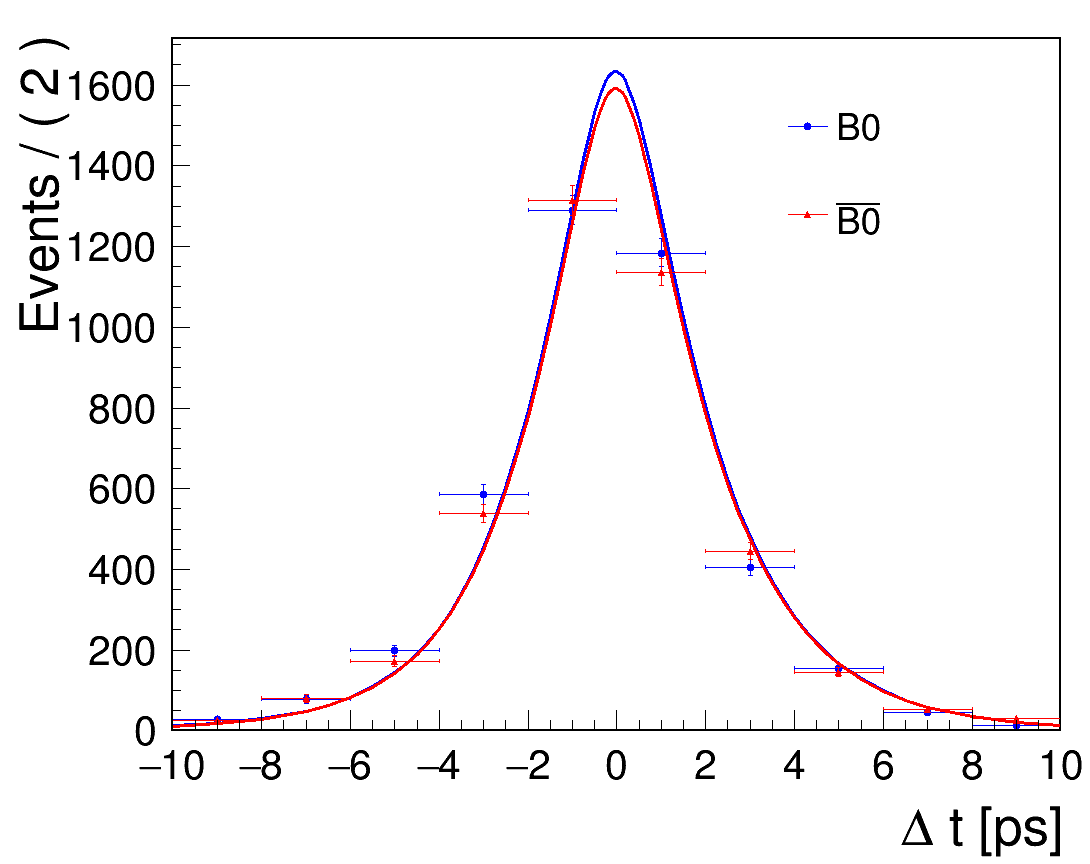
\includegraphics[height=5cm]{figures/cpfit-10000sig}
		\caption{$\it{CP}$ fit on 8873 signal MC.}
	\end{minipage}
	\begin{minipage}{0.5\linewidth}
		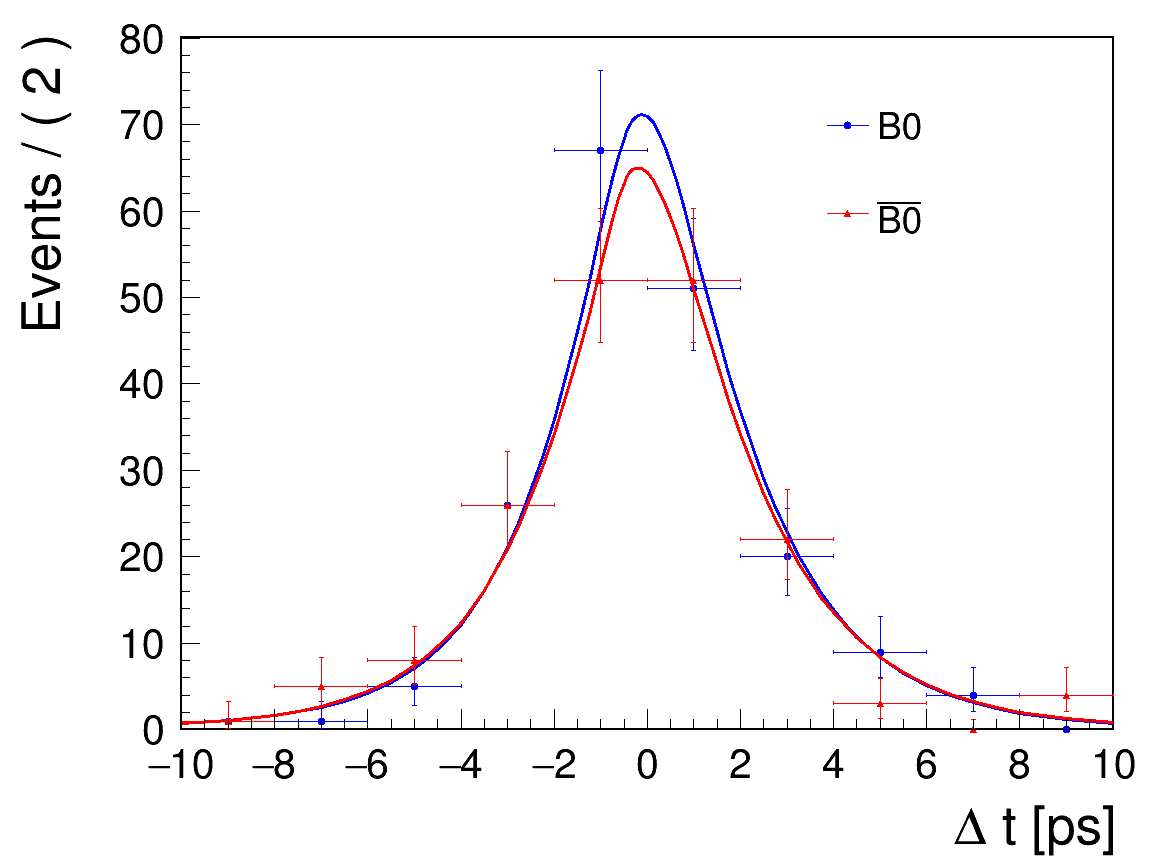
\includegraphics[height=5cm]{figures/cpfit-373gen}
		\caption{$\it{CP}$ fit on 373 generic MC.}
	\end{minipage}
	\begin{minipage}{0.5\linewidth}
		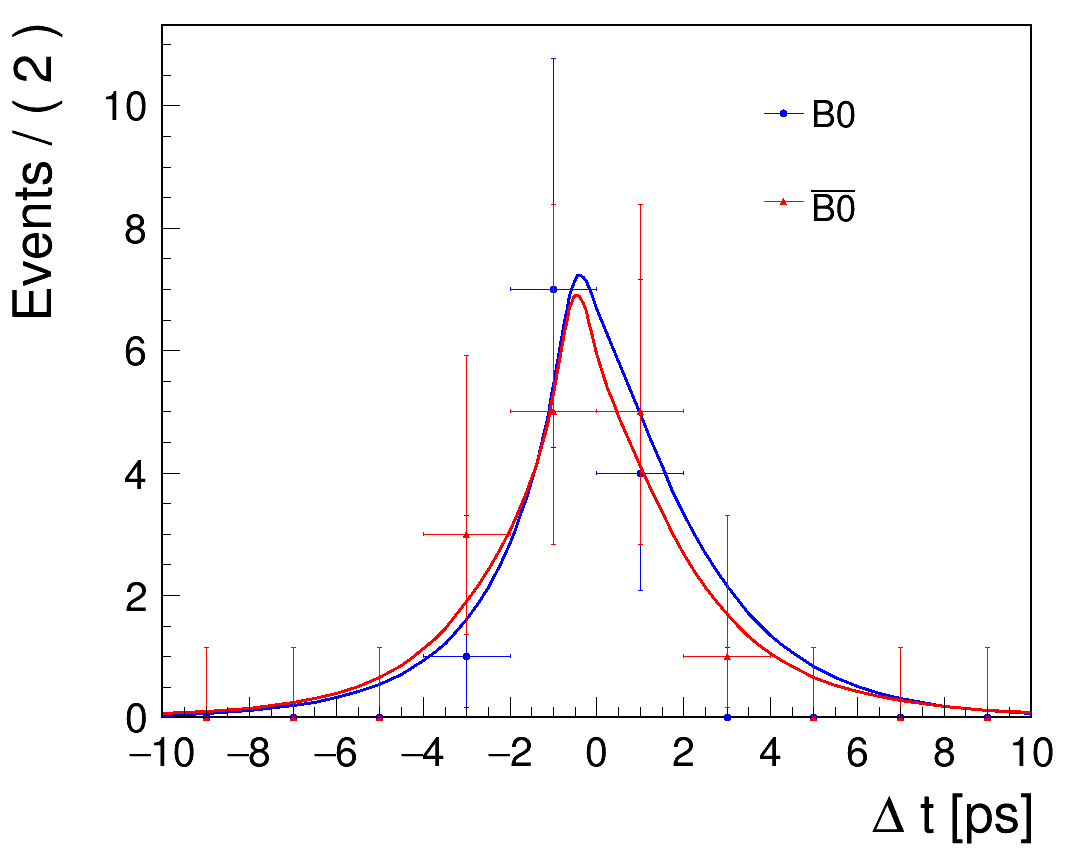
\includegraphics[height=5cm]{figures/cpfit-30gen}
		\caption{$\it{CP}$ fit on 30 generic MC.}
	\end{minipage}
\end{figure}

The fit result for 8873 signal MC is:
\begin{equation}
\begin{split}
sin(2\phi_1) & = 0.00 \pm 0.04 \\
\mathcal{A} & = -0.01 \pm 0.02\\
\end{split}
\end{equation} 
the fit result for 373 generic MC is:
\begin{equation}
\begin{split}
sin(2\phi_1) & = 0.00 \pm 0.21 \\
\mathcal{A} & = -0.05 \pm 0.07\\
\end{split}
\end{equation} 
the fit result for 30 events generic MC is:
\begin{equation}
\begin{split}
sin(2\phi_1) & = 0.20 \pm 0.85 \\
\mathcal{A} & = -0.06 \pm 0.30\\
\end{split}
\end{equation} 

The fit results are consistent with expectation in non-$\it{CP}$ violation from MC input, and the statistical uncertainties has the tendency $\delta \propto 1/\sqrt{N}$ as poission distribution. To test fit on non-zero $\it{CP}$ violating MC, the fit on $B^0\to J/\psi K_S^0$ signal MC is also done, the details of events selection as well as fit model determination can be found\cite{jpsiks_ichep}. The fit result over 10000 events is shown in FIG.30, which results in $sin(2\phi_1) = 0.70 \pm 0.05 $ and $\mathcal{A} = -0.01\pm 0.02$. The results agree with the input.
\begin{figure}[H]
	\centering
	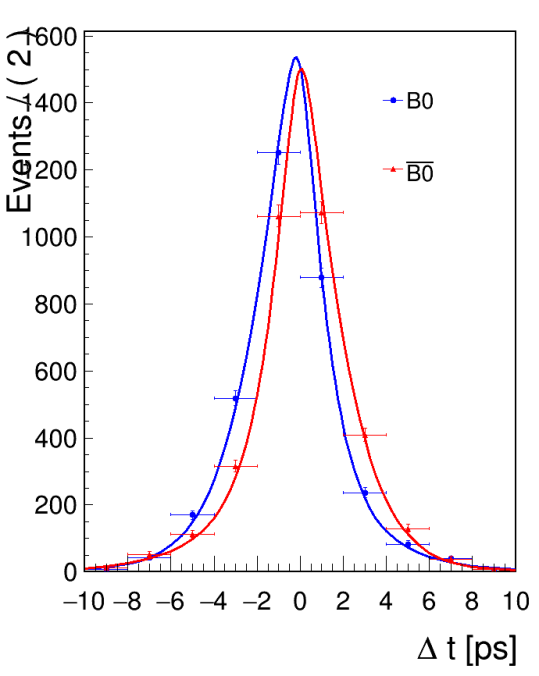
\includegraphics[height=5cm,width=5cm]{figures/jpsiks_cpfit10000}
	\caption{$\it{CP}$ fit over 10000 $B^0\to J/\psi K_S^0$ signal MC. }
\end{figure}
%We test the $\it{CP}$ fit on the sideband data with $M_{bc} < 5.27$ GeV.

\subsection{Linearity Test}
To validate the $\it{CP}$ fit linearity, we generate a series of toy MC sample, which the $\chi_2$, $N$ and vertex errors on $\it{CP}$ and tag-side are sampled from distribution of signal MC. The resolution functions parameters are kept same as MC fit as previous section. The input $\mathcal{A}$ is set to zero while the input value of $sin(2\phi_1)$ is running from 0.1 to 0.9. Each dataset contains 10000 events. The dependence between input and output are shown below. The linearity fit shows a good agreement between input and output.

\begin{figure}[H]
	\begin{minipage}{0.5\linewidth}
		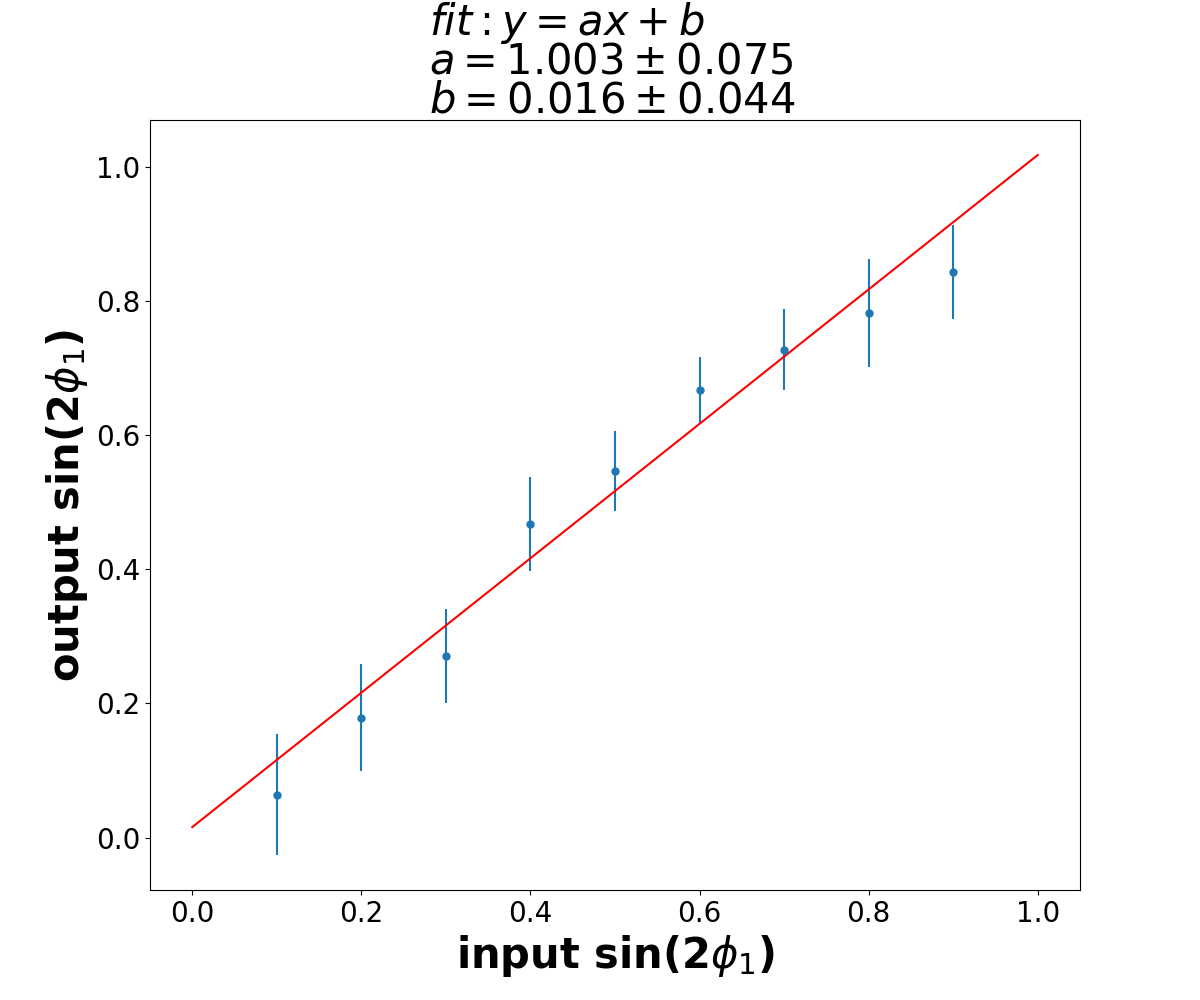
\includegraphics[height=6cm]{figures/S-test-line}
		%\caption{$\it{CP}$ fit on 8873 signal MC.}
	\end{minipage}
	\begin{minipage}{0.5\linewidth}
		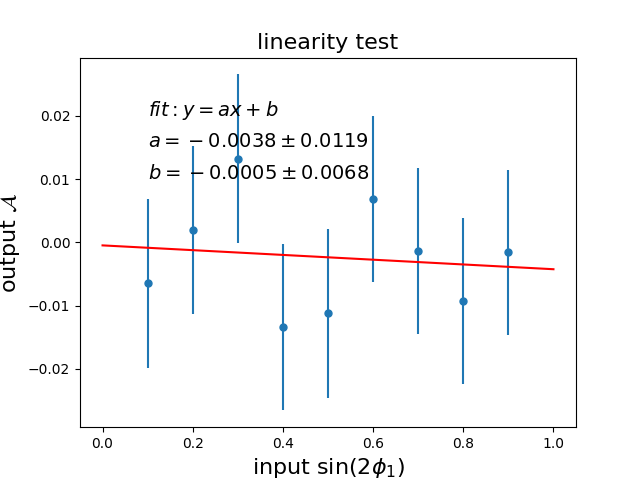
\includegraphics[height=6cm]{figures/A-test-line}
		%\caption{$\it{CP}$ fit on 373 generic MC.}
	\end{minipage}
	\caption{Linearity test of $\it{CP}$ fit.}
\end{figure}

Also, we fix  sin$(2\phi_1)$ at zero while floating $\mathcal{A}$ from  0.1 to 0.9, the dependence between input and output are as Fig 5-14 shows. The linearity fit shows a good agreement as well.
\begin{figure}[H]
	\begin{minipage}{0.5\linewidth}
		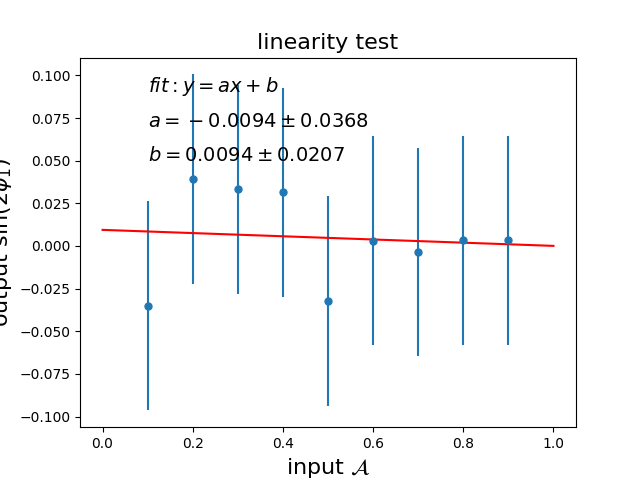
\includegraphics[height=6cm]{figures/S-test-line_fixS}
		%\caption{$\it{CP}$ fit on 8873 signal MC.}
	\end{minipage}
	\begin{minipage}{0.5\linewidth}
		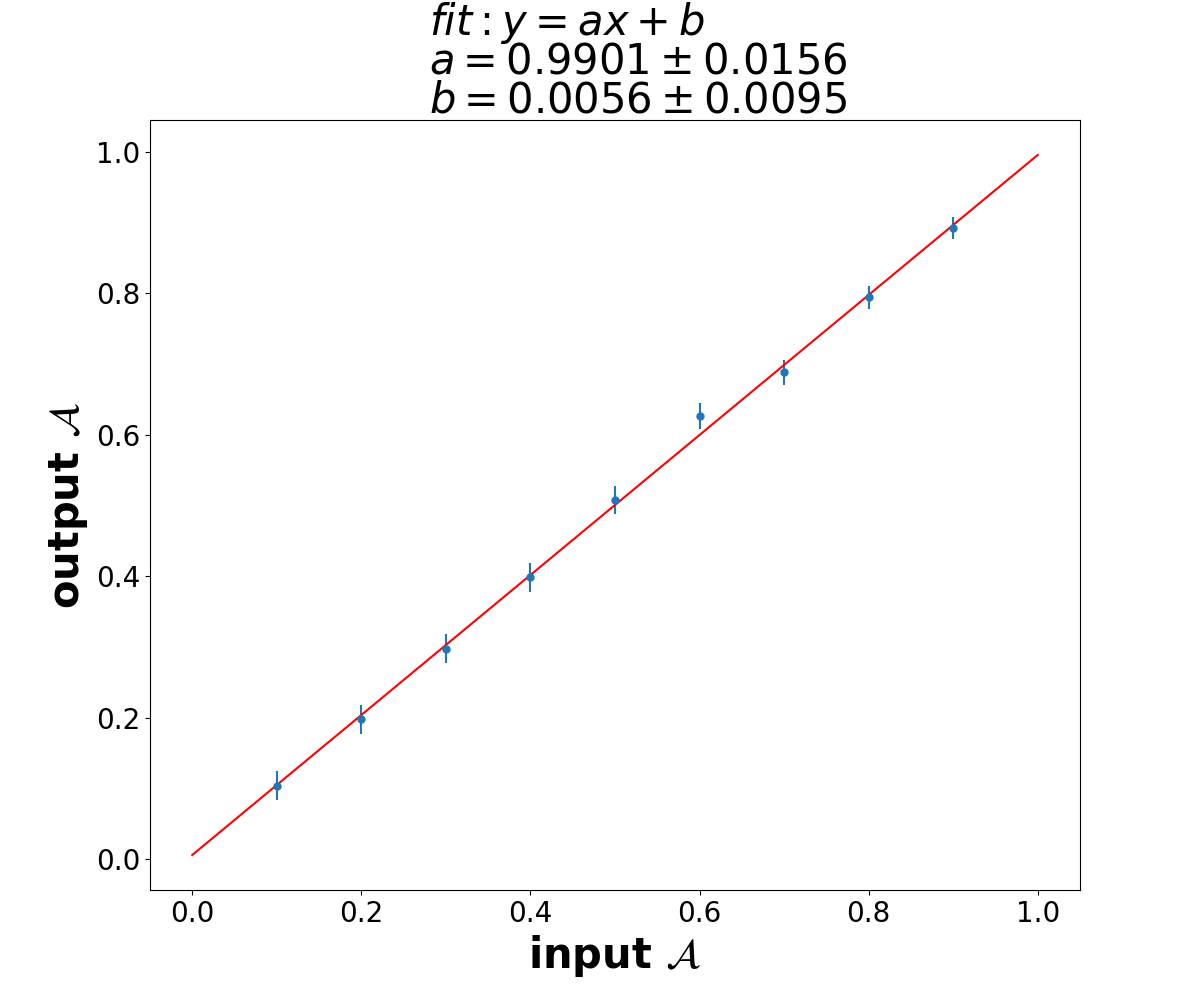
\includegraphics[height=6cm]{figures/A-test-line_fixS}
		%\caption{$\it{CP}$ fit on 373 generic MC.}
	\end{minipage}
	\caption{Linearity test of $\it{CP}$ fit.}
\end{figure}

\subsection{Toy MC Fit Pull}
In order to check the fit bias with input-output method, a series of 1000 dataset of toy MC has been created containing about 26 events in each. The event number is set based on the expected number from signal region in data after the selection.  $\chi_2$, $N$ and vertex errors on $\it{CP}$ and tag-side are sampled from distribution of data. The fit to dataset has only  sin(2$\phi_1$) and $\mathcal{A}$ as floating parameters, which input are both zero.
We expect to use normal distribution to describe the pull of sin(2$\phi_1$) and $\mathcal{A}$. 

\begin{figure}[H]
	\begin{minipage}{0.5\linewidth}
		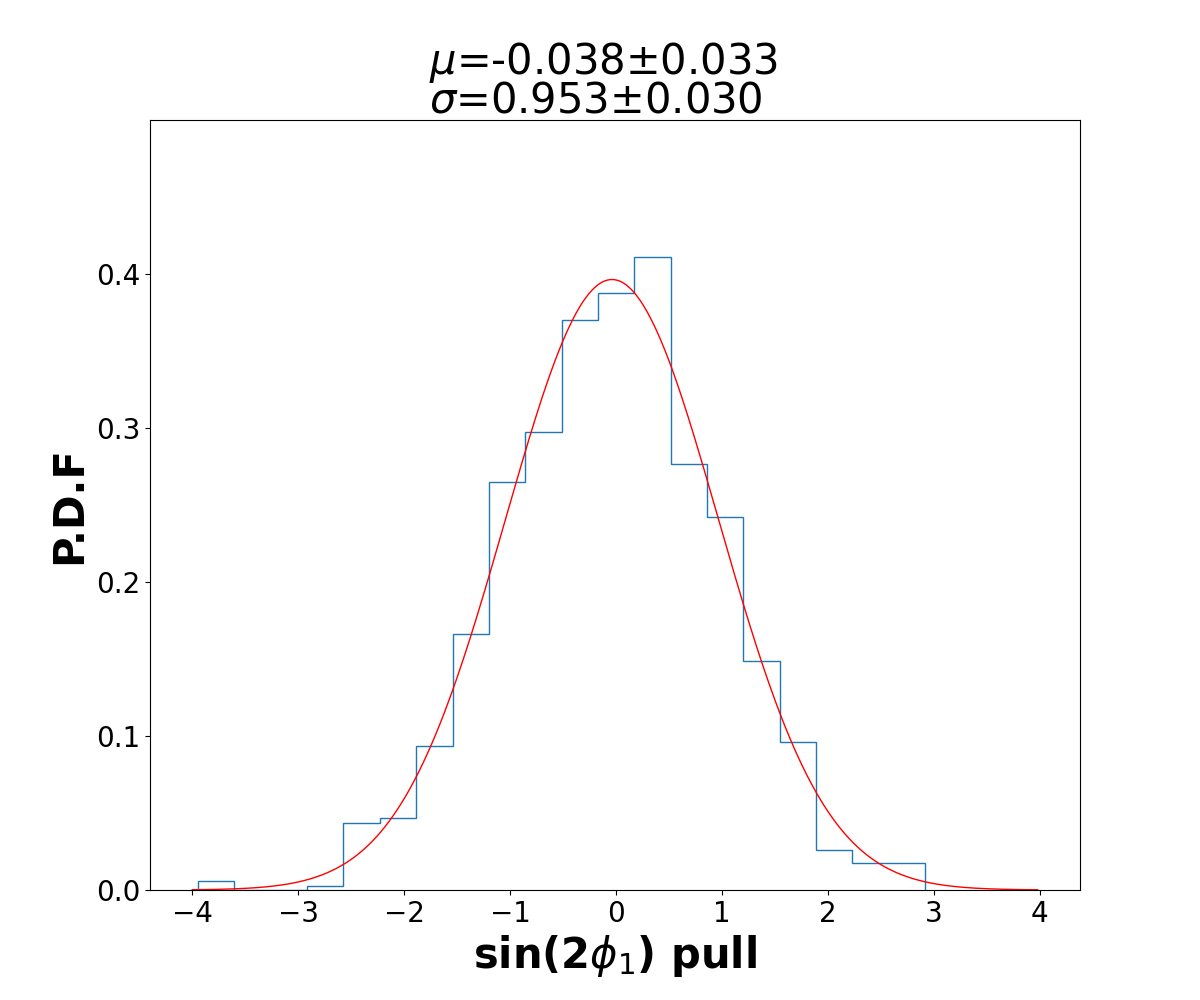
\includegraphics[height=6cm]{figures/pull_hist_S}
		%\caption{$\it{CP}$ fit on 8873 signal MC.}
	\end{minipage}
	\begin{minipage}{0.5\linewidth}
		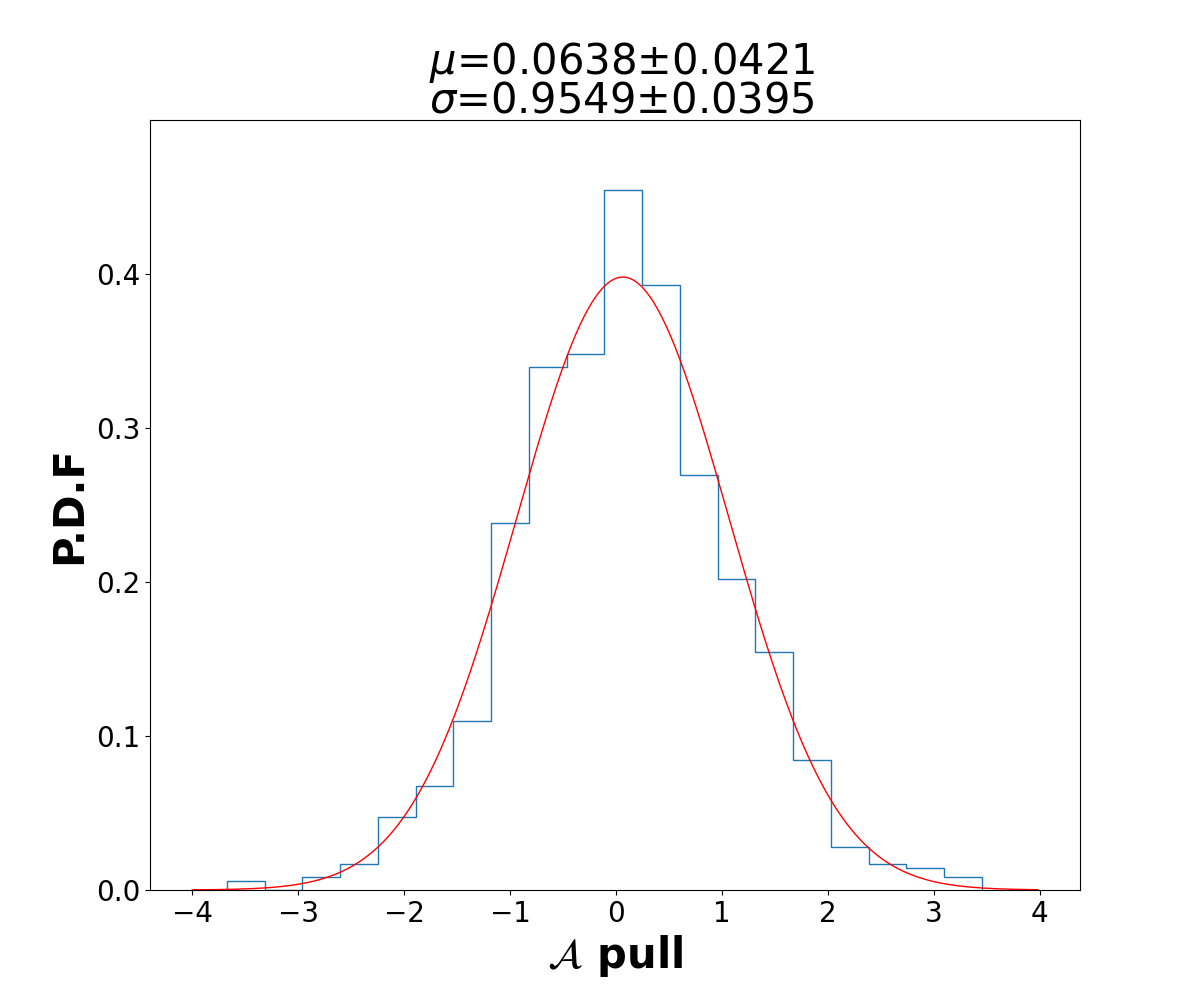
\includegraphics[height=6cm]{figures/pull_hist_A}
		%\caption{$\it{CP}$ fit on 373 generic MC.}
	\end{minipage}
	\caption{Pull of sin$(2\phi_1)$ and $\mathcal{A}$ fitted.}
\end{figure}

The fit results shows a good recovery of input sin$(2\phi_1)$ and $\mathcal{A}$ with no clear bias is spotted.


\subsection{Lifetime and $\Delta m_d$ Fit}
Before looking at $\it{CP}$ parameters in data, we need to check if the physics parameters are consistent when setting the $\it{CP}$ fitter to fit them in float. To test lifetime fit, first we use 10000 signal MC events which is generated by $\tau_{B^0} = 1.520$ from PDG value. The sin$(2\phi_1)$ and $\mathcal{A}$ are fixed at zero during the fit, for which the generator level $\it{CP}$ violation is zero. This is equivalent fit to:
\begin{equation}
\mathcal{P}(\Delta t,\tau_{B^0}) = 
\frac{e^{-|\Delta t|/\tau_{B^0}}}{4\tau_{B^0}}
\end{equation}
The fit result is $1.537 \pm 0.024$ ps which is consistent with the input. We perform the lifetime fit on data in signal region, the $\it{CP}$ parameters are fixed based on PDG values to: sin$(2\phi_1)=0.69$ and $\mathcal{A} = 0$. The fitted lifetime from $B^0 \to K_S^0  K_S^0  K_S^0$ is $1.431\pm 0.382$ ps. The result is consistent with PDG value. The distribution of $\Delta t$ in lifetime fit is shown as Fig 5-16.
The $B^0$ and $B^+$ lifetime fit using control sample is also performed and summarized in here\cite{jpsiks_ichep}. The results are consistent with PDG values. 
\begin{figure}[H]
	\centering
	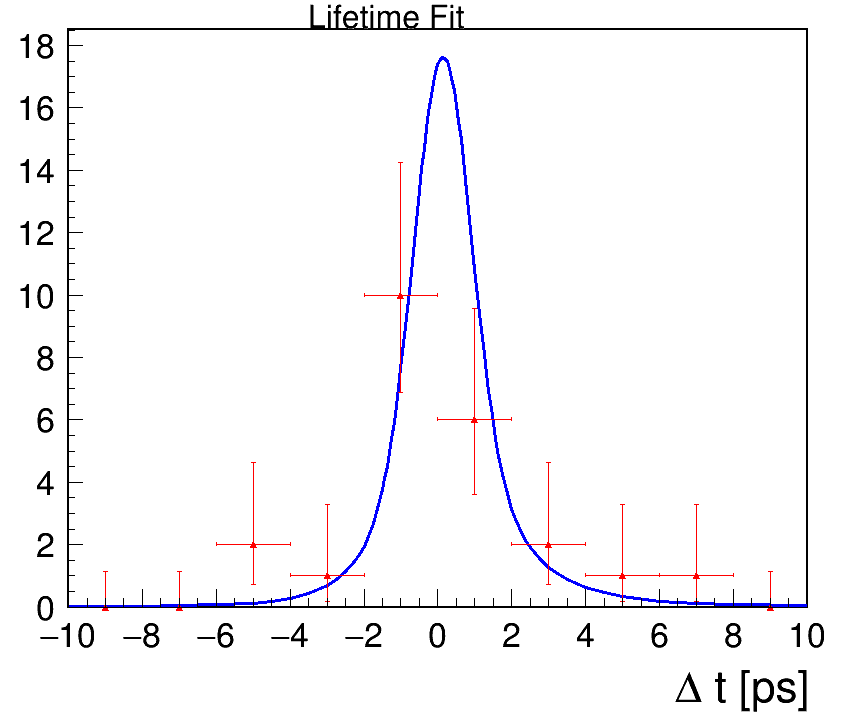
\includegraphics[height=7cm]{figures/lifetime_data}
	\caption{Lifetime fit on data}
\end{figure}
%\subsection{Control Sample fit}

To test the fit on physics parameter $\Delta m_d$, we generate 200 toy MC sets of $B^0 \to K_S^0  K_S^0  K_S^0$ with input $\Delta m_d = 0.507 $ GeV/$c^2$ where each set contains 26 events as same as data. The fit result is close to normal distribution and the pull of $\Delta m_d$ is shown in Fig 5-17. 
\begin{figure}[H]
	\centering
	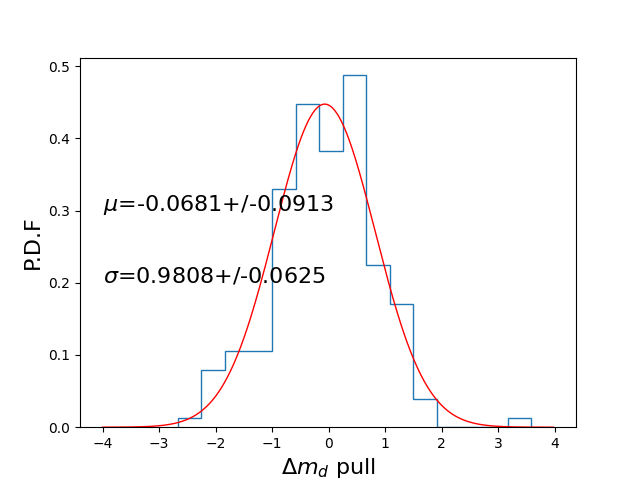
\includegraphics[height=7cm]{figures/pull_hist_dm}
	\caption{Pull of $\Delta m_d$}
\end{figure}
%\subsection{Control Sample fit}

\section{$\it{CP}$ fit on data}
After the $\it{CP}$ fit procedures from the previous sections 5.1 to 5.5 is reviewed by Belle II collaboration, the permission of measuring $\it{CP}$ parameters using Belle II 2019 and 2020 Spring/Summer data is granted by the review committee. The event number used for the $\it{CP}$ fit is 26, and the fit result is shown as: 

\begin{figure}[H]
	\centering
	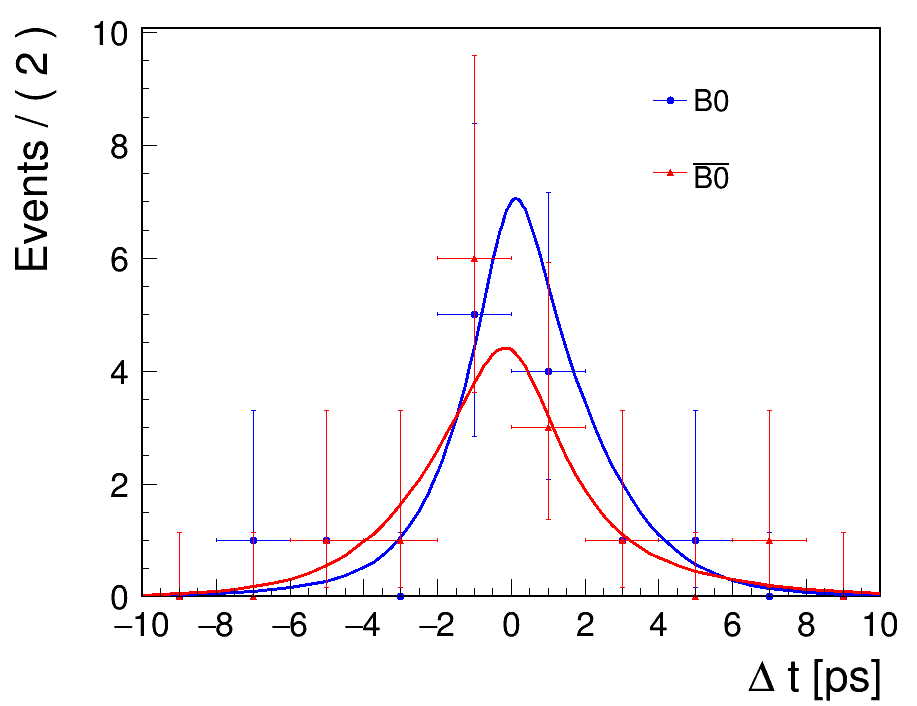
\includegraphics[height=6cm]{cpfit-data}
	\caption{The $\it{CP}$ fit from data.}
\end{figure}

The results of $\it{CP}$ parameters are: 

\begin{equation}
\begin{split}
sin(2\phi_1) & = 0.82 \pm 0.85(stat) \\
\mathcal{A} & = -0.21 \pm 0.28(stat) \\
\end{split}
\end{equation} 

\section{Systematic Uncertainty}
The systematic uncertainty that affects the fit results may come from many aspects of the measurement setup. 
In this measurement considering the options we used for signal extraction, vertexing and fit strategy, the major systematic uncertainty receives contribution from following points:

\begin{itemize}
	\item resolution functions parameters
	\item signal fraction
	\item flavor tagging 
	\item background $\Delta t$ shapes
	\item fit bias
	\item physics parameters
\end{itemize}
For the above sources of systematic uncertainty, if the parameters are defined with MC study, we float the value by $\pm 2 \sigma$ of their uncertainty, and if the parameters are defined by data, we float the value by $\pm 1 \sigma$, to have a more robust estimation of impact on fit results. The impact of $\it{CP}$ parameters are separately estimated from each sources with positive and negative differentials. With sum of the quadrature of each term, the overall systematic uncertainty is obtained. 

The signal resolution functions' parameters are determined from MC study for signal component. The impact on fit results is summarized as follows: 
\begin{table}[H]
	\begin{minipage}[b]{1.0\linewidth}
		\centering
		\caption{systematic uncertainty from resolution models}
		\begin{tabular}{c c c c c}
			\hline
			source & $+\delta \mathcal{S}$ & $+\delta \mathcal{A}$ & $-\delta \mathcal{S}$ &  $-\delta \mathcal{A}$\\
			$f_{cp}^{tail}$ & -0.000096 & -0.000057
			& 0.000014
			& 0.000056
			\\
			$s_0^{main}$& 0.005443
			& 0.001299
			& -0.005675
			& -0.001404
			\\
			$s_1^{main}$ & 0.019934
			& -0.000903
			& -0.020204
			& 0.000633
			\\
			$s_0^{tail}$ &  -0.003233
			& -0.001623
			& 0.00327
			& 0.001596
			\\
			$f_{tag}^{tail}$ & 0.00314
			& -0.001257
			& -0.003117
			& 0.001266
			\\
			$s_0^{main}$&  0.002011
			& -0.001395
			& -0.001956
			& 0.001398
			\\
			$s_1^{main}$ & 0.005059
			& -0.00084
			& -0.004969
			& 0.000825
			\\
			$s_0^{tail}$ &  -0.000135
			& -0.000393
			& 0.00010 & 0.000435
			\\
			$s_1^{tail}$  & 0.000101 & 0.000027 &  -0.000472
			& 0.000129
			\\
			$f_{\delta}$ & -0.007248
			& -0.000552
			& 0.007231
			& 0.000591
			\\
			$f_p$ &  0.003037
			& 0.004347
			& -0.003069
			& -0.004314
			\\
			$\tau_n$ & -0.00101 & -0.002841
			& 0.000937
			& 0.00294
			\\
			$\tau_p$ &  0.004497
			& 0.002502
			& -0.004648
			& -0.002478
			\\
			\hline
		\end{tabular}
	\end{minipage}
\end{table}
The background $\Delta t$ shapes' parameters are determined from data sideband $M_{bc}<5.26$ GeV. The impact on fit results is summarized as follows: 
\begin{table}[H]
	\begin{minipage}[b]{1.0\linewidth}
		\centering
		\caption{systematic uncertainty from background $\Delta t$ shapes}
		\begin{tabular}{c c c c c}
			\hline
			source & $+\delta \mathcal{S}$ & $+\delta \mathcal{A}$ & $-\delta \mathcal{S}$ &  $-\delta \mathcal{A}$\\
			$\mu^{bkg}_{\delta}$ & -0.014294
			& -0.016581
			& 0.006758
			& 0.006537
			\\
			$\mu^{bkg}_{l}$&  -0.002798
			& -0.012567
			& 0.003789
			& 0.012783
			\\
			$\tau_{bkg}$ & 0.001377
			& 0.001689
			& -0.004159
			& 0.000085\\
			$f_{\delta}^{bkg}$ &  -0.011315
			& 0.001365
			& 0.011187
			& -0.001395
			\\
			$f^{bkg}_{tail}$  &-0.002661
			& 0.00153
			& 0.00248
			& -0.001368
			\\
			$\sigma^{bkg}_{main}$ & 0.0207015
			& 0.022041
			& -0.0236175
			& -0.01569
			\\
			$\sigma^{bkg}_{tail}$ & -0.000275 & -0.000159
			& 0.000179
			& 0.000141
			\\
			\hline
		\end{tabular}
	\end{minipage}
\end{table}
The flavor tagging parameters wrong tagging fraction $ w$ in each rbin is determined from signal MC. The impact in each rbin on fit results is summarized as follows: 
\begin{table}[H]
	\begin{minipage}[b]{1.0\linewidth}
		\centering
		\caption{systematic uncertainty from wrong tagging fraction}
		\begin{tabular}{c c c c c}
			\hline
			source & $+\delta \mathcal{S}$ & $+\delta \mathcal{A}$ & $-\delta \mathcal{S}$ &  $-\delta \mathcal{A}$\\
			$w_1$ & -0.0018919
			& 0.001911
			& 0.0018549
			& -0.002004
			\\
			$ w_2$ & -0.0016448
			& 0.001104
			& 0.0016085
			& -0.001155
			\\
			$ w_3$ & -0.0004899
			& 0.001344
			& 0.0004726
			& -0.001341
			\\
			$ w_4$ & 0.0006556
			& 0.000264
			& -0.0006542
			& -0.000255 \\
			$ w_5$ & -0.0001228
			& 0.000204
			& 0.0001225 &
			-0.000195
			\\
			$ w_6$ & 0.0000948 & 0.000054 & 0.0000957 & -0.000045 \\
			$ w_7$ & 0.0001911
			& -0.000396
			& -0.0001907
			& 0.000402
			\\
			\hline
		\end{tabular}
	\end{minipage}
\end{table}
The physics parameters $\Delta m_d$ and $\tau_{B^0}$ uncertainties are included using the PDG average value. The impact on fit results is summarized as follows: 
\begin{table}[H]
	\begin{minipage}[b]{1.0\linewidth}
		\centering
		\caption{systematic uncertainty from  physics parameters}
		\begin{tabular}{c c c c c}
			\hline
			source & $+\delta \mathcal{S}$ & $+\delta \mathcal{A}$ & $-\delta \mathcal{S}$ &  $-\delta \mathcal{A}$\\
			$\Delta m_d$  & -0.001767
			& -0.000687
			& 0.001778
			& 0.000696
			\\
			$\tau_{B^0}$  & -0.004561
			& -0.000546
			& 0.004565
			& 0.000555
			\\
			\hline
		\end{tabular}
	\end{minipage}
\end{table}
The signal fraction is determined using 2D fit results of $M_{bc}$ and $\Delta E$ from data. The impact on fit results is summarized as follows: 
\begin{table}[H]
	\begin{minipage}[b]{1.0\linewidth}
		\centering
		\caption{systematic uncertainty from  signal fraction}
		\begin{tabular}{c c c c c}
			\hline
			source & $+\delta \mathcal{S}$ & $+\delta \mathcal{A}$ & $-\delta \mathcal{S}$ &  $-\delta \mathcal{A}$\\
			mu1\_mbc  & 0.000822 &	-0.003888&	-0.0007965&	0.003849
			\\
			sigma1\_mbc & 0.0004755&	0.008442&	-0.000628&	-0.008733
			\\
			m0\_argus & -0.000707&	0.00414	&0.001448&	-0.005781
			\\
			c\_argus & -0.005544&	0.001449&	0.000922&	-0.000078\\
			f1\_de & 0.0278255 &	0.020589&	-0.0192365	&-0.008409
			\\
			f2\_de & 0.020809&	0.017649	&-0.0161285	&-0.007005
			\\
			mu1\_de & -0.000443&	-0.000153&	0.0004955&	0.000088\\
			mu2\_de & -0.000563&	0.001446&	0.0005905&	-0.001446
			\\
			mu3\_de & -0.0031635&	-0.000834&	0.003354&	0.000981
			\\
			sigma1\_de& -0.0001715&	-0.000966&	0.000206&	0.000906
			\\
			sigma2\_de& -0.0031495&	0.002958&	0.0026345&	-0.002475
			\\
			sigma3\_de& -0.001926&	-0.00255&	0.0024695&	0.002985
			\\
			a0\_cheb & 0.0009515&	0.000057&	-0.0008925&	-0.000102
			\\
			N\_sig\_f & -0.0046395&	0.003987&	0.004922&	-0.003504
			\\
			\hline
		\end{tabular}
	\end{minipage}
\end{table}
The fit bias uncertainties is determined by the fit error of 100k signal MC events, which is $\delta {\mathcal{S}}=0.0098$ and $\delta {\mathcal{A}}=0.0057$.


\section{Summary}
The $\it{CP}$ parameters measurement study targeting the extraction of asymmetry parameters $\mathcal{S}$ and $\mathcal{A}$ has been conducted. Based on physical $\Delta t$ distribution, the model for $\it{CP}$ fit have been properly built. Importantly, corresponding resolution functions for $\mathcal{P}_{sig}$ and $\mathcal{P}_{bkg}$ are built by separating smearing effects from \textit{CP} and tag side. All the fits takes advantage of event-by-event conditional fit so the model has a good robustness in different measurement quality cases. As for flavor tagging, an algorithm based on FBDT classification is developed and implemented to give the estimated dilution factor $r$. To take a good use of these information, a Belle II $\it{CP}$ fitter is developed to perform the fit on desired parameters. The linearity test and fit pull test shows a reliable performance of the fitter using toy MC study. The actual fit on lifetime using data is also consistent with the PDG value with a relatively large uncertainty due to very small amount of data. 

After the blind fit and test for the $\it{CP}$ parameters measurement is conduced, with the permission from Belle II collaboration, we unblind the data in signal box and perform the $\it{CP}$ fit to extract $\mathcal{S}$ and $\mathcal{A}$. Also, the major sources of systematic uncertainty is estimated. The primary result of $\it{CP}$ parameters in this low luminosity stage are:

\begin{equation}
\begin{split}
\mathcal{S}=- sin(2\phi_1) & = -0.82 \pm 0.85(stat) \pm 0.07(syst) \\
\mathcal{A} & = -0.21\pm 0.28(stat) \pm 0.06(syst)\\
\end{split}
\end{equation}  

The results are dominated by the statistical uncertainty due to the very limited data sample in early stage of Belle II. Under such large uncertainty, the results is in an agreement with the Standard Model. 


